% Judul dokumen
\title{Buku Tugas Akhir ITS}
\author{Setiadi Ekatama, I Putu Haris}

% Pengaturan ukuran teks dan bentuk halaman dua sisi
\documentclass[12pt,twoside]{report}

% Pengaturan ukuran halaman dan margin
\usepackage[a4paper,top=30mm,left=30mm,right=20mm,bottom=25mm]{geometry}

% Pengaturan ukuran spasi
\usepackage[singlespacing]{setspace}

% Pengaturan detail pada file PDF
\usepackage[pdfauthor={\@author},bookmarksnumbered,pdfborder={0 0 0}]{hyperref}

% Pengaturan jenis karakter
\usepackage[utf8]{inputenc}

% Pengaturan pewarnaan
\usepackage[table,xcdraw]{xcolor}

% Pengaturan kutipan artikel
\usepackage[style=apa, backend=biber]{biblatex}

% Package lainnya
\usepackage{changepage}
\usepackage{enumitem}
\usepackage{eso-pic}
\usepackage{txfonts} % Font times
\usepackage{etoolbox}
\usepackage{graphicx}
\usepackage{lipsum}
\usepackage{longtable}
\usepackage{tabularx}
\usepackage{wrapfig}
\usepackage{float}

% Definisi untuk "Hati ini sengaja dikosongkan"
\patchcmd{\cleardoublepage}{\hbox{}}{
  \thispagestyle{empty}
  \vspace*{\fill}
  \begin{center}\textit{[Halaman ini sengaja dikosongkan]}\end{center}
  \vfill}{}{}

% Pengaturan penomoran halaman
\usepackage{fancyhdr}
\fancyhf{}
\renewcommand{\headrulewidth}{0pt}
\pagestyle{fancy}
\fancyfoot[LE,RO]{\thepage}
\patchcmd{\chapter}{plain}{fancy}{}{}
\patchcmd{\chapter}{empty}{plain}{}{}

% Command untuk bulan
\newcommand{\MONTH}{%
  \ifcase\the\month
  \or Januari% 1
  \or Februari% 2
  \or Maret% 3
  \or April% 4
  \or Mei% 5
  \or Juni% 6
  \or Juli% 7
  \or Agustus% 8
  \or September% 9
  \or Oktober% 10
  \or November% 11
  \or Desember% 12
  \fi}
\newcommand{\ENGMONTH}{%
  \ifcase\the\month
  \or January% 1
  \or February% 2
  \or March% 3
  \or April% 4
  \or May% 5
  \or June% 6
  \or July% 7
  \or August% 8
  \or September% 9
  \or October% 10
  \or November% 11
  \or December% 12
  \fi}

% Pengaturan format judul bab
\usepackage{titlesec}
\titleformat{\chapter}[display]{\bfseries\Large}{BAB \centering\Roman{chapter}}{0ex}{\vspace{0ex}\centering}
\titleformat{\section}{\bfseries\large}{\MakeUppercase{\thesection}}{1ex}{\vspace{1ex}}
\titleformat{\subsection}{\bfseries\large}{\MakeUppercase{\thesubsection}}{1ex}{}
\titleformat{\subsubsection}{\bfseries\large}{\MakeUppercase{\thesubsubsection}}{1ex}{}
\titlespacing{\chapter}{0ex}{0ex}{4ex}
\titlespacing{\section}{0ex}{1ex}{0ex}
\titlespacing{\subsection}{0ex}{0.5ex}{0ex}
\titlespacing{\subsubsection}{0ex}{0.5ex}{0ex}

% Atur variabel berikut sesuai namanya

% nama
\newcommand{\name}{I Putu Haris Setiadi Ekatama}
\newcommand{\authorname}{Setiadi Ekatama, I Putu Haris}
\newcommand{\nickname}{Haris}
\newcommand{\advisor}{Dr. Eko Mulyanto Yuniarno, S.T., M.T.}
% \newcommand{\coadvisor}{-}
\newcommand{\examinerone}{Dion Hayu Fandiantoro, S.T., M.Eng.}
\newcommand{\examinertwo}{Dr. Arief Kurniawan, S.T., M.T.}
\newcommand{\examinerthree}{Arta Kusuma Hernanda, S.T., M.T.}
\newcommand{\headofdepartment}{Dr. Supeno Mardi Susiki Nugroho, S.T., M.T.}

% identitas
\newcommand{\nrp}{0721 19 4000 0046}
\newcommand{\advisornip}{19680601 199512 1 009}
% \newcommand{\coadvisornip}{-}
\newcommand{\examineronenip}{19942020 11064}
\newcommand{\examinertwonip}{19740907 200212 1 001}
\newcommand{\examinerthreenip}{19962023 11024}
\newcommand{\headofdepartmentnip}{19700313 199512 1 001}

% judul
\newcommand{\tatitle}{PERANCANGAN SISTEM KONTROL MOTOR KURSI RODA SECARA NIRKABEL BERBASIS ESP32}
\newcommand{\engtatitle}{\emph{DESIGNING A WIRELESS CONTROL SYSTEM FOR WHEELCHAIR MOTORS BASED ON ESP32}}

% tempat
\newcommand{\place}{Surabaya}

% jurusan
\newcommand{\studyprogram}{Teknik Komputer}
\newcommand{\engstudyprogram}{Computer Engineering}

% fakultas
\newcommand{\faculty}{Teknologi Elektro dan Informatika Cerdas}
\newcommand{\engfaculty}{Intelligent Electrical and Informatics Technology}

% singkatan fakultas
\newcommand{\facultyshort}{FTEIC}
\newcommand{\engfacultyshort}{F-ELECTICS}

% departemen
\newcommand{\department}{Teknik Komputer}
\newcommand{\engdepartment}{Computer Engineering}

% kode mata kuliah
\newcommand{\coursecode}{EC234801}

% Tambahkan format tanda hubung yang benar di sini
\hyphenation{
  da-lam
  te-ro-bo-san
  ro-ket
  me-ngem-bang-kan
  per-hi-tu-ngan
  tek-no-lo-gi
  me-la-ku-kan
  ber-so-si-al-i-sa-si
  ke-lum-pu-han
  be-ru-pa
  wak-tu
  di-da-pat-kan
  me-ngi-rim-kan
  pe-ngi-ri-man
  pe-ngu-ji-an
  me-nun-juk-kan
  me-la-lui
  ji-ka
  ter-hu-bung
  ter-da-pat
  meng-hu-bung-kan-nya
  me-ru-pa-kan
  me-ngi-rim-kan
  di-gu-na-kan
  add-ress
}

% Menambahkan resource daftar pustaka
\addbibresource{pustaka/pustaka.bib}

% Pengaturan format potongan kode
\usepackage{listings}
\definecolor{comment}{RGB}{0,128,0}
\definecolor{string}{RGB}{255,0,0}
\definecolor{keyword}{RGB}{0,0,255}
\lstdefinestyle{codestyle}{
  commentstyle=\color{comment},
  stringstyle=\color{string},
  keywordstyle=\color{keyword},
  basicstyle=\fontsize{12}{14}\ttfamily,
  numbers=left,
  numberstyle=\fontsize{12}{14},
  numbersep=5pt,
  frame=lines,
  breaklines=true,
  prebreak=\raisebox{0ex}[0ex][0ex]{\ensuremath{\hookleftarrow}},
  showstringspaces=false,
  upquote=true,
  tabsize=2,
}
\lstset{style=codestyle}

% Penambahan Bahasa Pemrograman Arduino
 %%%%%%%%%%%%%%%%%%%%%%%%%%%%%%%%%%%%%%%%%%%%%%%%%%%%%%%%%%%%%%%%%%%%%%%%%%%%%%%% 
%%% ~ Arduino Language - Arduino IDE Colors ~                                  %%%
%%%                                                                            %%%
%%% Kyle Rocha-Brownell | 10/2/2017 | No Licence                               %%%
%%% -------------------------------------------------------------------------- %%%
%%%                                                                            %%%
%%% Place this file in your working directory (next to the latex file you're   %%%
%%% working on).  To add it to your project, place:                            %%%
%%%     %%%%%%%%%%%%%%%%%%%%%%%%%%%%%%%%%%%%%%%%%%%%%%%%%%%%%%%%%%%%%%%%%%%%%%%%%%%%%%%% 
%%% ~ Arduino Language - Arduino IDE Colors ~                                  %%%
%%%                                                                            %%%
%%% Kyle Rocha-Brownell | 10/2/2017 | No Licence                               %%%
%%% -------------------------------------------------------------------------- %%%
%%%                                                                            %%%
%%% Place this file in your working directory (next to the latex file you're   %%%
%%% working on).  To add it to your project, place:                            %%%
%%%     %%%%%%%%%%%%%%%%%%%%%%%%%%%%%%%%%%%%%%%%%%%%%%%%%%%%%%%%%%%%%%%%%%%%%%%%%%%%%%%% 
%%% ~ Arduino Language - Arduino IDE Colors ~                                  %%%
%%%                                                                            %%%
%%% Kyle Rocha-Brownell | 10/2/2017 | No Licence                               %%%
%%% -------------------------------------------------------------------------- %%%
%%%                                                                            %%%
%%% Place this file in your working directory (next to the latex file you're   %%%
%%% working on).  To add it to your project, place:                            %%%
%%%    \input{arduinoLanguage.tex}                                             %%%
%%% somewhere before \begin{document} in your latex file.                      %%%
%%%                                                                            %%%
%%% In your document, place your arduino code between:                         %%%
%%%   \begin{lstlisting}[language=Arduino]                                     %%%
%%% and:                                                                       %%%
%%%   \end{lstlisting}                                                         %%%
%%%                                                                            %%%
%%% Or create your own style to add non-built-in functions and variables.      %%%
%%%                                                                            %%%
 %%%%%%%%%%%%%%%%%%%%%%%%%%%%%%%%%%%%%%%%%%%%%%%%%%%%%%%%%%%%%%%%%%%%%%%%%%%%%%%% 

 \usepackage{color}
 \usepackage{listings}    
 \usepackage{courier}
 
 %%% Define Custom IDE Colors %%%
 \definecolor{arduinoGreen}    {rgb} {0.17, 0.43, 0.01}
 \definecolor{arduinoGrey}     {rgb} {0.47, 0.47, 0.33}
 \definecolor{arduinoOrange}   {rgb} {0.8 , 0.4 , 0   }
 \definecolor{arduinoBlue}     {rgb} {0.01, 0.61, 0.98}
 \definecolor{arduinoDarkBlue} {rgb} {0.0 , 0.2 , 0.5 }
 \definecolor{arduinoBlack}    {rgb} {0.0 , 0.0 , 0.0}
 
 %%% Define Arduino Language %%%
 \lstdefinelanguage{Arduino}{
   language=C++, % begin with default C++ settings 
 %
 %
   %%% Keyword Color Group 1 %%%  (called KEYWORD3 by arduino)
   keywordstyle=\color{arduinoGreen},   
   deletekeywords={  % remove all arduino keywords that might be in c++
                 break, case, override, final, continue, default, do, else, for, 
                 if, return, goto, switch, throw, try, while, setup, loop, export, 
                 not, or, and, xor, include, define, elif, else, error, if, ifdef, 
                 ifndef, pragma, warning,
                 HIGH, LOW, INPUT, INPUT_PULLUP, OUTPUT, DEC, BIN, HEX, OCT, PI, 
                 HALF_PI, TWO_PI, LSBFIRST, MSBFIRST, CHANGE, FALLING, RISING, 
                 DEFAULT, EXTERNAL, INTERNAL, INTERNAL1V1, INTERNAL2V56, LED_BUILTIN, 
                 LED_BUILTIN_RX, LED_BUILTIN_TX, DIGITAL_MESSAGE, FIRMATA_STRING, 
                 ANALOG_MESSAGE, REPORT_DIGITAL, REPORT_ANALOG, SET_PIN_MODE, 
                 SYSTEM_RESET, SYSEX_START, auto, int8_t, int16_t, int32_t, int64_t, 
                 uint8_t, uint16_t, uint32_t, uint64_t, char16_t, char32_t, operator, 
                 enum, delete, bool, boolean, byte, char, const, false, float, double, 
                 null, NULL, int, long, new, private, protected, public, short, 
                 signed, static, volatile, String, void, true, unsigned, word, array, 
                 sizeof, dynamic_cast, typedef, const_cast, struct, static_cast, union, 
                 friend, extern, class, reinterpret_cast, register, explicit, inline, 
                 _Bool, complex, _Complex, _Imaginary, atomic_bool, atomic_char, 
                 atomic_schar, atomic_uchar, atomic_short, atomic_ushort, atomic_int, 
                 atomic_uint, atomic_long, atomic_ulong, atomic_llong, atomic_ullong, 
                 virtual, PROGMEM,
                 Serial, Serial1, Serial2, Serial3, SerialUSB, Keyboard, Mouse,
                 abs, acos, asin, atan, atan2, ceil, constrain, cos, degrees, exp, 
                 floor, log, map, max, min, radians, random, randomSeed, round, sin, 
                 sq, sqrt, tan, pow, bitRead, bitWrite, bitSet, bitClear, bit, 
                 highByte, lowByte, analogReference, analogRead, 
                 analogReadResolution, analogWrite, analogWriteResolution, 
                 attachInterrupt, detachInterrupt, digitalPinToInterrupt, delay, 
                 delayMicroseconds, digitalWrite, digitalRead, interrupts, millis, 
                 micros, noInterrupts, noTone, pinMode, pulseIn, pulseInLong, shiftIn, 
                 shiftOut, tone, yield, Stream, begin, end, peek, read, print, 
                 println, available, availableForWrite, flush, setTimeout, find, 
                 findUntil, parseInt, parseFloat, readBytes, readBytesUntil, readString, 
                 readStringUntil, trim, toUpperCase, toLowerCase, charAt, compareTo, 
                 concat, endsWith, startsWith, equals, equalsIgnoreCase, getBytes, 
                 indexOf, lastIndexOf, length, replace, setCharAt, substring, 
                 toCharArray, toInt, press, release, releaseAll, accept, click, move, 
                 isPressed, isAlphaNumeric, isAlpha, isAscii, isWhitespace, isControl, 
                 isDigit, isGraph, isLowerCase, isPrintable, isPunct, isSpace, 
                 isUpperCase, isHexadecimalDigit, 
                 }, 
   morekeywords={   % add arduino structures to group 1
                 break, case, override, final, continue, default, do, else, for, 
                 if, return, goto, switch, throw, try, while, setup, loop, export, 
                 not, or, and, xor, include, define, elif, else, error, if, ifdef, 
                 ifndef, pragma, warning,
                 }, 
 % 
 %
   %%% Keyword Color Group 2 %%%  (called LITERAL1 by arduino)
   keywordstyle=[2]\color{arduinoBlue},   
   keywords=[2]{   % add variables and dataTypes as 2nd group  
                 HIGH, LOW, INPUT, INPUT_PULLUP, OUTPUT, DEC, BIN, HEX, OCT, PI, 
                 HALF_PI, TWO_PI, LSBFIRST, MSBFIRST, CHANGE, FALLING, RISING, 
                 DEFAULT, EXTERNAL, INTERNAL, INTERNAL1V1, INTERNAL2V56, LED_BUILTIN, 
                 LED_BUILTIN_RX, LED_BUILTIN_TX, DIGITAL_MESSAGE, FIRMATA_STRING, 
                 ANALOG_MESSAGE, REPORT_DIGITAL, REPORT_ANALOG, SET_PIN_MODE, 
                 SYSTEM_RESET, SYSEX_START, auto, int8_t, int16_t, int32_t, int64_t, 
                 uint8_t, uint16_t, uint32_t, uint64_t, char16_t, char32_t, operator, 
                 enum, delete, bool, boolean, byte, char, const, false, float, double, 
                 null, NULL, int, long, new, private, protected, public, short, 
                 signed, static, volatile, String, void, true, unsigned, word, array, 
                 sizeof, dynamic_cast, typedef, const_cast, struct, static_cast, union, 
                 friend, extern, class, reinterpret_cast, register, explicit, inline, 
                 _Bool, complex, _Complex, _Imaginary, atomic_bool, atomic_char, 
                 atomic_schar, atomic_uchar, atomic_short, atomic_ushort, atomic_int, 
                 atomic_uint, atomic_long, atomic_ulong, atomic_llong, atomic_ullong, 
                 virtual, PROGMEM,
                 },  
 % 
 %
   %%% Keyword Color Group 3 %%%  (called KEYWORD1 by arduino)
   keywordstyle=[3]\bfseries\color{arduinoOrange},
   keywords=[3]{  % add built-in functions as a 3rd group
                 Serial, Serial1, Serial2, Serial3, SerialUSB, Keyboard, Mouse,
                 },      
 %
 %
   %%% Keyword Color Group 4 %%%  (called KEYWORD2 by arduino)
   keywordstyle=[4]\color{arduinoOrange},
   keywords=[4]{  % add more built-in functions as a 4th group
                 abs, acos, asin, atan, atan2, ceil, constrain, cos, degrees, exp, 
                 floor, log, map, max, min, radians, random, randomSeed, round, sin, 
                 sq, sqrt, tan, pow, bitRead, bitWrite, bitSet, bitClear, bit, 
                 highByte, lowByte, analogReference, analogRead, 
                 analogReadResolution, analogWrite, analogWriteResolution, 
                 attachInterrupt, detachInterrupt, digitalPinToInterrupt, delay, 
                 delayMicroseconds, digitalWrite, digitalRead, interrupts, millis, 
                 micros, noInterrupts, noTone, pinMode, pulseIn, pulseInLong, shiftIn, 
                 shiftOut, tone, yield, Stream, begin, end, peek, read, print, 
                 println, available, availableForWrite, flush, setTimeout, find, 
                 findUntil, parseInt, parseFloat, readBytes, readBytesUntil, readString, 
                 readStringUntil, trim, toUpperCase, toLowerCase, charAt, compareTo, 
                 concat, endsWith, startsWith, equals, equalsIgnoreCase, getBytes, 
                 indexOf, lastIndexOf, length, replace, setCharAt, substring, 
                 toCharArray, toInt, press, release, releaseAll, accept, click, move, 
                 isPressed, isAlphaNumeric, isAlpha, isAscii, isWhitespace, isControl, 
                 isDigit, isGraph, isLowerCase, isPrintable, isPunct, isSpace, 
                 isUpperCase, isHexadecimalDigit, 
                 },      
 %
 %
   %%% Set Other Colors %%%
   stringstyle=\color{arduinoDarkBlue},    
   commentstyle=\color{arduinoGrey},    
 %          
 %   
   %%%% Line Numbering %%%%
   numbers=left,                    
   numbersep=5pt,                   
   numberstyle=\color{arduinoBlack},    
   %stepnumber=2,                      % show every 2 line numbers
 %
 %
   %%%% Code Box Style %%%%
   breaklines=true,                    % wordwrapping
   tabsize=2,         
   basicstyle=\ttfamily  
 }                                             %%%
%%% somewhere before \begin{document} in your latex file.                      %%%
%%%                                                                            %%%
%%% In your document, place your arduino code between:                         %%%
%%%   \begin{lstlisting}[language=Arduino]                                     %%%
%%% and:                                                                       %%%
%%%   \end{lstlisting}                                                         %%%
%%%                                                                            %%%
%%% Or create your own style to add non-built-in functions and variables.      %%%
%%%                                                                            %%%
 %%%%%%%%%%%%%%%%%%%%%%%%%%%%%%%%%%%%%%%%%%%%%%%%%%%%%%%%%%%%%%%%%%%%%%%%%%%%%%%% 

 \usepackage{color}
 \usepackage{listings}    
 \usepackage{courier}
 
 %%% Define Custom IDE Colors %%%
 \definecolor{arduinoGreen}    {rgb} {0.17, 0.43, 0.01}
 \definecolor{arduinoGrey}     {rgb} {0.47, 0.47, 0.33}
 \definecolor{arduinoOrange}   {rgb} {0.8 , 0.4 , 0   }
 \definecolor{arduinoBlue}     {rgb} {0.01, 0.61, 0.98}
 \definecolor{arduinoDarkBlue} {rgb} {0.0 , 0.2 , 0.5 }
 \definecolor{arduinoBlack}    {rgb} {0.0 , 0.0 , 0.0}
 
 %%% Define Arduino Language %%%
 \lstdefinelanguage{Arduino}{
   language=C++, % begin with default C++ settings 
 %
 %
   %%% Keyword Color Group 1 %%%  (called KEYWORD3 by arduino)
   keywordstyle=\color{arduinoGreen},   
   deletekeywords={  % remove all arduino keywords that might be in c++
                 break, case, override, final, continue, default, do, else, for, 
                 if, return, goto, switch, throw, try, while, setup, loop, export, 
                 not, or, and, xor, include, define, elif, else, error, if, ifdef, 
                 ifndef, pragma, warning,
                 HIGH, LOW, INPUT, INPUT_PULLUP, OUTPUT, DEC, BIN, HEX, OCT, PI, 
                 HALF_PI, TWO_PI, LSBFIRST, MSBFIRST, CHANGE, FALLING, RISING, 
                 DEFAULT, EXTERNAL, INTERNAL, INTERNAL1V1, INTERNAL2V56, LED_BUILTIN, 
                 LED_BUILTIN_RX, LED_BUILTIN_TX, DIGITAL_MESSAGE, FIRMATA_STRING, 
                 ANALOG_MESSAGE, REPORT_DIGITAL, REPORT_ANALOG, SET_PIN_MODE, 
                 SYSTEM_RESET, SYSEX_START, auto, int8_t, int16_t, int32_t, int64_t, 
                 uint8_t, uint16_t, uint32_t, uint64_t, char16_t, char32_t, operator, 
                 enum, delete, bool, boolean, byte, char, const, false, float, double, 
                 null, NULL, int, long, new, private, protected, public, short, 
                 signed, static, volatile, String, void, true, unsigned, word, array, 
                 sizeof, dynamic_cast, typedef, const_cast, struct, static_cast, union, 
                 friend, extern, class, reinterpret_cast, register, explicit, inline, 
                 _Bool, complex, _Complex, _Imaginary, atomic_bool, atomic_char, 
                 atomic_schar, atomic_uchar, atomic_short, atomic_ushort, atomic_int, 
                 atomic_uint, atomic_long, atomic_ulong, atomic_llong, atomic_ullong, 
                 virtual, PROGMEM,
                 Serial, Serial1, Serial2, Serial3, SerialUSB, Keyboard, Mouse,
                 abs, acos, asin, atan, atan2, ceil, constrain, cos, degrees, exp, 
                 floor, log, map, max, min, radians, random, randomSeed, round, sin, 
                 sq, sqrt, tan, pow, bitRead, bitWrite, bitSet, bitClear, bit, 
                 highByte, lowByte, analogReference, analogRead, 
                 analogReadResolution, analogWrite, analogWriteResolution, 
                 attachInterrupt, detachInterrupt, digitalPinToInterrupt, delay, 
                 delayMicroseconds, digitalWrite, digitalRead, interrupts, millis, 
                 micros, noInterrupts, noTone, pinMode, pulseIn, pulseInLong, shiftIn, 
                 shiftOut, tone, yield, Stream, begin, end, peek, read, print, 
                 println, available, availableForWrite, flush, setTimeout, find, 
                 findUntil, parseInt, parseFloat, readBytes, readBytesUntil, readString, 
                 readStringUntil, trim, toUpperCase, toLowerCase, charAt, compareTo, 
                 concat, endsWith, startsWith, equals, equalsIgnoreCase, getBytes, 
                 indexOf, lastIndexOf, length, replace, setCharAt, substring, 
                 toCharArray, toInt, press, release, releaseAll, accept, click, move, 
                 isPressed, isAlphaNumeric, isAlpha, isAscii, isWhitespace, isControl, 
                 isDigit, isGraph, isLowerCase, isPrintable, isPunct, isSpace, 
                 isUpperCase, isHexadecimalDigit, 
                 }, 
   morekeywords={   % add arduino structures to group 1
                 break, case, override, final, continue, default, do, else, for, 
                 if, return, goto, switch, throw, try, while, setup, loop, export, 
                 not, or, and, xor, include, define, elif, else, error, if, ifdef, 
                 ifndef, pragma, warning,
                 }, 
 % 
 %
   %%% Keyword Color Group 2 %%%  (called LITERAL1 by arduino)
   keywordstyle=[2]\color{arduinoBlue},   
   keywords=[2]{   % add variables and dataTypes as 2nd group  
                 HIGH, LOW, INPUT, INPUT_PULLUP, OUTPUT, DEC, BIN, HEX, OCT, PI, 
                 HALF_PI, TWO_PI, LSBFIRST, MSBFIRST, CHANGE, FALLING, RISING, 
                 DEFAULT, EXTERNAL, INTERNAL, INTERNAL1V1, INTERNAL2V56, LED_BUILTIN, 
                 LED_BUILTIN_RX, LED_BUILTIN_TX, DIGITAL_MESSAGE, FIRMATA_STRING, 
                 ANALOG_MESSAGE, REPORT_DIGITAL, REPORT_ANALOG, SET_PIN_MODE, 
                 SYSTEM_RESET, SYSEX_START, auto, int8_t, int16_t, int32_t, int64_t, 
                 uint8_t, uint16_t, uint32_t, uint64_t, char16_t, char32_t, operator, 
                 enum, delete, bool, boolean, byte, char, const, false, float, double, 
                 null, NULL, int, long, new, private, protected, public, short, 
                 signed, static, volatile, String, void, true, unsigned, word, array, 
                 sizeof, dynamic_cast, typedef, const_cast, struct, static_cast, union, 
                 friend, extern, class, reinterpret_cast, register, explicit, inline, 
                 _Bool, complex, _Complex, _Imaginary, atomic_bool, atomic_char, 
                 atomic_schar, atomic_uchar, atomic_short, atomic_ushort, atomic_int, 
                 atomic_uint, atomic_long, atomic_ulong, atomic_llong, atomic_ullong, 
                 virtual, PROGMEM,
                 },  
 % 
 %
   %%% Keyword Color Group 3 %%%  (called KEYWORD1 by arduino)
   keywordstyle=[3]\bfseries\color{arduinoOrange},
   keywords=[3]{  % add built-in functions as a 3rd group
                 Serial, Serial1, Serial2, Serial3, SerialUSB, Keyboard, Mouse,
                 },      
 %
 %
   %%% Keyword Color Group 4 %%%  (called KEYWORD2 by arduino)
   keywordstyle=[4]\color{arduinoOrange},
   keywords=[4]{  % add more built-in functions as a 4th group
                 abs, acos, asin, atan, atan2, ceil, constrain, cos, degrees, exp, 
                 floor, log, map, max, min, radians, random, randomSeed, round, sin, 
                 sq, sqrt, tan, pow, bitRead, bitWrite, bitSet, bitClear, bit, 
                 highByte, lowByte, analogReference, analogRead, 
                 analogReadResolution, analogWrite, analogWriteResolution, 
                 attachInterrupt, detachInterrupt, digitalPinToInterrupt, delay, 
                 delayMicroseconds, digitalWrite, digitalRead, interrupts, millis, 
                 micros, noInterrupts, noTone, pinMode, pulseIn, pulseInLong, shiftIn, 
                 shiftOut, tone, yield, Stream, begin, end, peek, read, print, 
                 println, available, availableForWrite, flush, setTimeout, find, 
                 findUntil, parseInt, parseFloat, readBytes, readBytesUntil, readString, 
                 readStringUntil, trim, toUpperCase, toLowerCase, charAt, compareTo, 
                 concat, endsWith, startsWith, equals, equalsIgnoreCase, getBytes, 
                 indexOf, lastIndexOf, length, replace, setCharAt, substring, 
                 toCharArray, toInt, press, release, releaseAll, accept, click, move, 
                 isPressed, isAlphaNumeric, isAlpha, isAscii, isWhitespace, isControl, 
                 isDigit, isGraph, isLowerCase, isPrintable, isPunct, isSpace, 
                 isUpperCase, isHexadecimalDigit, 
                 },      
 %
 %
   %%% Set Other Colors %%%
   stringstyle=\color{arduinoDarkBlue},    
   commentstyle=\color{arduinoGrey},    
 %          
 %   
   %%%% Line Numbering %%%%
   numbers=left,                    
   numbersep=5pt,                   
   numberstyle=\color{arduinoBlack},    
   %stepnumber=2,                      % show every 2 line numbers
 %
 %
   %%%% Code Box Style %%%%
   breaklines=true,                    % wordwrapping
   tabsize=2,         
   basicstyle=\ttfamily  
 }                                             %%%
%%% somewhere before \begin{document} in your latex file.                      %%%
%%%                                                                            %%%
%%% In your document, place your arduino code between:                         %%%
%%%   \begin{lstlisting}[language=Arduino]                                     %%%
%%% and:                                                                       %%%
%%%   \end{lstlisting}                                                         %%%
%%%                                                                            %%%
%%% Or create your own style to add non-built-in functions and variables.      %%%
%%%                                                                            %%%
 %%%%%%%%%%%%%%%%%%%%%%%%%%%%%%%%%%%%%%%%%%%%%%%%%%%%%%%%%%%%%%%%%%%%%%%%%%%%%%%% 

 \usepackage{color}
 \usepackage{listings}    
 \usepackage{courier}
 
 %%% Define Custom IDE Colors %%%
 \definecolor{arduinoGreen}    {rgb} {0.17, 0.43, 0.01}
 \definecolor{arduinoGrey}     {rgb} {0.47, 0.47, 0.33}
 \definecolor{arduinoOrange}   {rgb} {0.8 , 0.4 , 0   }
 \definecolor{arduinoBlue}     {rgb} {0.01, 0.61, 0.98}
 \definecolor{arduinoDarkBlue} {rgb} {0.0 , 0.2 , 0.5 }
 \definecolor{arduinoBlack}    {rgb} {0.0 , 0.0 , 0.0}
 
 %%% Define Arduino Language %%%
 \lstdefinelanguage{Arduino}{
   language=C++, % begin with default C++ settings 
 %
 %
   %%% Keyword Color Group 1 %%%  (called KEYWORD3 by arduino)
   keywordstyle=\color{arduinoGreen},   
   deletekeywords={  % remove all arduino keywords that might be in c++
                 break, case, override, final, continue, default, do, else, for, 
                 if, return, goto, switch, throw, try, while, setup, loop, export, 
                 not, or, and, xor, include, define, elif, else, error, if, ifdef, 
                 ifndef, pragma, warning,
                 HIGH, LOW, INPUT, INPUT_PULLUP, OUTPUT, DEC, BIN, HEX, OCT, PI, 
                 HALF_PI, TWO_PI, LSBFIRST, MSBFIRST, CHANGE, FALLING, RISING, 
                 DEFAULT, EXTERNAL, INTERNAL, INTERNAL1V1, INTERNAL2V56, LED_BUILTIN, 
                 LED_BUILTIN_RX, LED_BUILTIN_TX, DIGITAL_MESSAGE, FIRMATA_STRING, 
                 ANALOG_MESSAGE, REPORT_DIGITAL, REPORT_ANALOG, SET_PIN_MODE, 
                 SYSTEM_RESET, SYSEX_START, auto, int8_t, int16_t, int32_t, int64_t, 
                 uint8_t, uint16_t, uint32_t, uint64_t, char16_t, char32_t, operator, 
                 enum, delete, bool, boolean, byte, char, const, false, float, double, 
                 null, NULL, int, long, new, private, protected, public, short, 
                 signed, static, volatile, String, void, true, unsigned, word, array, 
                 sizeof, dynamic_cast, typedef, const_cast, struct, static_cast, union, 
                 friend, extern, class, reinterpret_cast, register, explicit, inline, 
                 _Bool, complex, _Complex, _Imaginary, atomic_bool, atomic_char, 
                 atomic_schar, atomic_uchar, atomic_short, atomic_ushort, atomic_int, 
                 atomic_uint, atomic_long, atomic_ulong, atomic_llong, atomic_ullong, 
                 virtual, PROGMEM,
                 Serial, Serial1, Serial2, Serial3, SerialUSB, Keyboard, Mouse,
                 abs, acos, asin, atan, atan2, ceil, constrain, cos, degrees, exp, 
                 floor, log, map, max, min, radians, random, randomSeed, round, sin, 
                 sq, sqrt, tan, pow, bitRead, bitWrite, bitSet, bitClear, bit, 
                 highByte, lowByte, analogReference, analogRead, 
                 analogReadResolution, analogWrite, analogWriteResolution, 
                 attachInterrupt, detachInterrupt, digitalPinToInterrupt, delay, 
                 delayMicroseconds, digitalWrite, digitalRead, interrupts, millis, 
                 micros, noInterrupts, noTone, pinMode, pulseIn, pulseInLong, shiftIn, 
                 shiftOut, tone, yield, Stream, begin, end, peek, read, print, 
                 println, available, availableForWrite, flush, setTimeout, find, 
                 findUntil, parseInt, parseFloat, readBytes, readBytesUntil, readString, 
                 readStringUntil, trim, toUpperCase, toLowerCase, charAt, compareTo, 
                 concat, endsWith, startsWith, equals, equalsIgnoreCase, getBytes, 
                 indexOf, lastIndexOf, length, replace, setCharAt, substring, 
                 toCharArray, toInt, press, release, releaseAll, accept, click, move, 
                 isPressed, isAlphaNumeric, isAlpha, isAscii, isWhitespace, isControl, 
                 isDigit, isGraph, isLowerCase, isPrintable, isPunct, isSpace, 
                 isUpperCase, isHexadecimalDigit, 
                 }, 
   morekeywords={   % add arduino structures to group 1
                 break, case, override, final, continue, default, do, else, for, 
                 if, return, goto, switch, throw, try, while, setup, loop, export, 
                 not, or, and, xor, include, define, elif, else, error, if, ifdef, 
                 ifndef, pragma, warning,
                 }, 
 % 
 %
   %%% Keyword Color Group 2 %%%  (called LITERAL1 by arduino)
   keywordstyle=[2]\color{arduinoBlue},   
   keywords=[2]{   % add variables and dataTypes as 2nd group  
                 HIGH, LOW, INPUT, INPUT_PULLUP, OUTPUT, DEC, BIN, HEX, OCT, PI, 
                 HALF_PI, TWO_PI, LSBFIRST, MSBFIRST, CHANGE, FALLING, RISING, 
                 DEFAULT, EXTERNAL, INTERNAL, INTERNAL1V1, INTERNAL2V56, LED_BUILTIN, 
                 LED_BUILTIN_RX, LED_BUILTIN_TX, DIGITAL_MESSAGE, FIRMATA_STRING, 
                 ANALOG_MESSAGE, REPORT_DIGITAL, REPORT_ANALOG, SET_PIN_MODE, 
                 SYSTEM_RESET, SYSEX_START, auto, int8_t, int16_t, int32_t, int64_t, 
                 uint8_t, uint16_t, uint32_t, uint64_t, char16_t, char32_t, operator, 
                 enum, delete, bool, boolean, byte, char, const, false, float, double, 
                 null, NULL, int, long, new, private, protected, public, short, 
                 signed, static, volatile, String, void, true, unsigned, word, array, 
                 sizeof, dynamic_cast, typedef, const_cast, struct, static_cast, union, 
                 friend, extern, class, reinterpret_cast, register, explicit, inline, 
                 _Bool, complex, _Complex, _Imaginary, atomic_bool, atomic_char, 
                 atomic_schar, atomic_uchar, atomic_short, atomic_ushort, atomic_int, 
                 atomic_uint, atomic_long, atomic_ulong, atomic_llong, atomic_ullong, 
                 virtual, PROGMEM,
                 },  
 % 
 %
   %%% Keyword Color Group 3 %%%  (called KEYWORD1 by arduino)
   keywordstyle=[3]\bfseries\color{arduinoOrange},
   keywords=[3]{  % add built-in functions as a 3rd group
                 Serial, Serial1, Serial2, Serial3, SerialUSB, Keyboard, Mouse,
                 },      
 %
 %
   %%% Keyword Color Group 4 %%%  (called KEYWORD2 by arduino)
   keywordstyle=[4]\color{arduinoOrange},
   keywords=[4]{  % add more built-in functions as a 4th group
                 abs, acos, asin, atan, atan2, ceil, constrain, cos, degrees, exp, 
                 floor, log, map, max, min, radians, random, randomSeed, round, sin, 
                 sq, sqrt, tan, pow, bitRead, bitWrite, bitSet, bitClear, bit, 
                 highByte, lowByte, analogReference, analogRead, 
                 analogReadResolution, analogWrite, analogWriteResolution, 
                 attachInterrupt, detachInterrupt, digitalPinToInterrupt, delay, 
                 delayMicroseconds, digitalWrite, digitalRead, interrupts, millis, 
                 micros, noInterrupts, noTone, pinMode, pulseIn, pulseInLong, shiftIn, 
                 shiftOut, tone, yield, Stream, begin, end, peek, read, print, 
                 println, available, availableForWrite, flush, setTimeout, find, 
                 findUntil, parseInt, parseFloat, readBytes, readBytesUntil, readString, 
                 readStringUntil, trim, toUpperCase, toLowerCase, charAt, compareTo, 
                 concat, endsWith, startsWith, equals, equalsIgnoreCase, getBytes, 
                 indexOf, lastIndexOf, length, replace, setCharAt, substring, 
                 toCharArray, toInt, press, release, releaseAll, accept, click, move, 
                 isPressed, isAlphaNumeric, isAlpha, isAscii, isWhitespace, isControl, 
                 isDigit, isGraph, isLowerCase, isPrintable, isPunct, isSpace, 
                 isUpperCase, isHexadecimalDigit, 
                 },      
 %
 %
   %%% Set Other Colors %%%
   stringstyle=\color{arduinoDarkBlue},    
   commentstyle=\color{arduinoGrey},    
 %          
 %   
   %%%% Line Numbering %%%%
   numbers=left,                    
   numbersep=5pt,                   
   numberstyle=\color{arduinoBlack},    
   %stepnumber=2,                      % show every 2 line numbers
 %
 %
   %%%% Code Box Style %%%%
   breaklines=true,                    % wordwrapping
   tabsize=2,         
   basicstyle=\ttfamily  
 }

% Isi keseluruhan dokumen
\begin{document}

% Sampul luar Bahasa Indonesia
\newcommand\covercontents{sampul/konten-id.tex}
\AddToShipoutPictureBG*{
  \AtPageLowerLeft{
    % Ubah nilai berikut jika posisi horizontal background tidak sesuai
    \hspace{-3.25mm}

    % Ubah nilai berikut jika posisi vertikal background tidak sesuai
    \raisebox{0mm}{
      
\includegraphics[width=\paperwidth,height=\paperheight]{sampul/gambar/sampul-luar.png}
    }
  }
}

% Menyembunyikan nomor halaman
\thispagestyle{empty}

% Pengaturan margin untuk menyesuaikan konten sampul
\newgeometry{
  top=55mm,
  left=30mm,
  right=20mm,
  bottom=20mm
}

\begin{flushleft}

  % Pemilihan font sans serif
  \sffamily

  % Pemilihan warna font putih
  \color{white}

  % Pemilihan font bold
  \fontseries{bx}
  \selectfont
  \begin{spacing}{1.5}
    \input{\covercontents}
  \end{spacing}

\end{flushleft}

\restoregeometry

\cleardoublepage

% Atur ulang penomoran halaman
\setcounter{page}{1}

% Sampul dalam Bahasa Indonesia
\renewcommand\covercontents{sampul/konten-id.tex}
\AddToShipoutPictureBG*{
  \AtPageLowerLeft{
    % Ubah nilai berikut jika posisi horizontal background tidak sesuai
    \hspace{-4mm}

    % Ubah nilai berikut jika posisi vertikal background tidak sesuai
    \raisebox{0mm}{
      
\includegraphics[width=\paperwidth,height=\paperheight]{sampul/gambar/sampul-luar-tipis.png}
    }
  }
}

% Menyembunyikan nomor halaman
\thispagestyle{empty}

% Pengaturan margin untuk menyesuaikan konten sampul
\newgeometry{
  top=65mm,
  left=30mm,
  right=30mm,
  bottom=20mm
}

\begin{flushleft}

  % Pemilihan font sans serif
  \sffamily

  % Pemilihan font bold
  \fontseries{bx}
  \selectfont
  \begin{spacing}{1.5}
    \input{\covercontents}
  \end{spacing}

\end{flushleft}

\restoregeometry

\clearpage
\cleardoublepage

% Sampul dalam Bahasa Inggris
\renewcommand\covercontents{sampul/konten-en.tex}
\AddToShipoutPictureBG*{
  \AtPageLowerLeft{
    % Ubah nilai berikut jika posisi horizontal background tidak sesuai
    \hspace{-4mm}

    % Ubah nilai berikut jika posisi vertikal background tidak sesuai
    \raisebox{0mm}{
      
\includegraphics[width=\paperwidth,height=\paperheight]{sampul/gambar/sampul-luar-tipis.png}
    }
  }
}

% Menyembunyikan nomor halaman
\thispagestyle{empty}

% Pengaturan margin untuk menyesuaikan konten sampul
\newgeometry{
  top=65mm,
  left=30mm,
  right=30mm,
  bottom=20mm
}

\begin{flushleft}

  % Pemilihan font sans serif
  \sffamily

  % Pemilihan font bold
  \fontseries{bx}
  \selectfont
  \begin{spacing}{1.5}
    \input{\covercontents}
  \end{spacing}

\end{flushleft}

\restoregeometry

\cleardoublepage

% Label tabel dan gambar dalam bahasa indonesia
\renewcommand{\figurename}{Gambar}
\renewcommand{\tablename}{Tabel}
\renewcommand{\lstlistingname}{Program}

% Pengaturan ukuran indentasi paragraf
\setlength{\parindent}{2em}

% Pengaturan ukuran spasi paragraf
\setlength{\parskip}{1ex}

% Lembar pengesahan
\begin{center}
  \large
  \textbf{LEMBAR PENGESAHAN}
\end{center}

% Menyembunyikan nomor halaman
\thispagestyle{empty}

\begin{center}
  \textbf{\tatitle{}}
\end{center}

\begingroup
% Pemilihan font ukuran small
\small

\begin{center}
  \textbf{TUGAS AKHIR}
  \\Diajukan untuk memenuhi salah satu syarat \\
  memperoleh gelar Sarjana Teknik pada \\
  Program Studi S-1 \studyprogram{} \\
  Departemen \department{} \\
  Fakultas \faculty{} \\
  Institut Teknologi Sepuluh Nopember
\end{center}

\begin{center}
  Oleh: \textbf{\name{}}
  \\NRP. \nrp{}
\end{center}

\begin{center}
  Disetujui oleh Tim Penguji Tugas Akhir:
\end{center}

\begingroup
% Menghilangkan padding
\setlength{\tabcolsep}{0pt}

\noindent
\begin{tabularx}{\textwidth}{X l}
  \advisor{}               & (Pembimbing I)                      \\
  NIP: \advisornip{}       &                                     \\
                           & ................................... \\
                           &                                     \\
                           &                                     \\
  %\coadvisor{}             & (Pembimbing II)                     \\
  %NIP: \coadvisornip{}     &                                     \\
  %                         & ................................... \\
  %                         &                                     \\
  %                        &                                     \\
  \examinerone{}.          & (Penguji I)                         \\
  NIP: \examineronenip{}   &                                     \\
                           & ................................... \\
                           &                                     \\
                           &                                     \\
  \examinertwo{}.          & (Penguji II)                        \\
  NIP: \examinertwonip{}   &                                     \\
                           & ................................... \\
                           &                                     \\
                           &                                     \\
  \examinerthree{}.        & (Penguji III)                       \\
  NIP: \examinerthreenip{} &                                     \\
                           & ................................... \\
\end{tabularx}
\endgroup

\begin{center}
  Mengetahui, \\
  Kepala Departemen \department{} \facultyshort{} - ITS\\

  \vspace{8ex}

  \underline{\headofdepartment{}.} \\
  NIP. \headofdepartmentnip{}
\end{center}

\begin{center}
  \textbf{\MakeUppercase{\place{}}\\\MONTH{}, \the\year{}}
\end{center}
\endgroup

\cleardoublepage
\begin{center}
  \large
  \textbf{APPROVAL SHEET}
\end{center}

% Menyembunyikan nomor halaman
\thispagestyle{empty}

\begin{center}
  \textbf{\engtatitle{}}
\end{center}

\begingroup
% Pemilihan font ukuran small
\small

\begin{center}
  \textbf{FINAL PROJECT}
  \\Submitted to fulfill one of the requirements \\
  for obtaining a degree Bachelor of Engineering at \\
  Undergraduate Study Program of \engstudyprogram{} \\
  Department of \engdepartment{} \\
  Faculty of \engfaculty{} \\
  Sepuluh Nopember Institute of Technology
\end{center}

\begin{center}
  By: \textbf{\name{}}
  \\NRP. \nrp{}
\end{center}

\begin{center}
  Approved by Final Project Examiner Team:
\end{center}

\begingroup
% Menghilangkan padding
\setlength{\tabcolsep}{0pt}

\noindent
\begin{tabularx}{\textwidth}{X l}
  \advisor{}               & (Advisor I)                         \\
  NIP: \advisornip{}       &                                     \\
                           & ................................... \\
                           &                                     \\
                           &                                     \\
  %\coadvisor{}             & (Co-Advisor II)                     \\
  %NIP: \coadvisornip{}     &                                     \\
  %                         & ................................... \\
  %                         &                                     \\
  %                         &                                     \\
  \examinerone{}.          & (Examiner I)                        \\
  NIP: \examineronenip{}   &                                     \\
                           & ................................... \\
                           &                                     \\
                           &                                     \\
  \examinertwo{}.          & (Examiner II)                       \\
  NIP: \examinertwonip{}   &                                     \\
                           & ................................... \\
                           &                                     \\
                           &                                     \\
  \examinerthree{}.        & (Examiner III)                      \\
  NIP: \examinerthreenip{} &                                     \\
                           & ................................... \\
\end{tabularx}
\endgroup


\begin{center}
  Acknowledged, \\
  Head of \engdepartment{} Department \engfacultyshort{} - ITS \\

  \vspace{8ex}

  \underline{\headofdepartment{}.} \\
  NIP. \headofdepartmentnip{}
\end{center}

\begin{center}
  \textbf{\MakeUppercase{\place{}}\\\ENGMONTH{}, \the\year{}}
\end{center}
\endgroup

\cleardoublepage

% Pernyataan keaslian
\begin{center}
  \large
  \textbf{PERNYATAAN ORISINALITAS}
\end{center}

% Menyembunyikan nomor halaman
\thispagestyle{empty}

\vspace{2ex}

% Ubah paragraf-paragraf berikut sesuai dengan yang ingin diisi pada pernyataan keaslian

\noindent Yang bertanda tangan dibawah ini:

\noindent\begin{tabularx}{\textwidth}{l l X}
                         &   &                            \\
  Nama Mahasiswa / NRP   & : & \name{} / \nrp{}           \\
  Departemen             & : & \department{}              \\
  Dosen Pembimbing / NIP & : & \advisor{} / \advisornip{} \\
                         &   &                            \\
\end{tabularx}

Dengan ini menyatakan bahwa Tugas Akhir dengan judul "\tatitle{}" adalah hasil karya sendiri, berfsifat orisinal, dan ditulis dengan mengikuti kaidah penulisan ilmiah.

Bilamana di kemudian hari ditemukan ketidaksesuaian dengan pernyataan ini, maka saya bersedia menerima sanksi sesuai dengan ketentuan yang berlaku di Institut Teknologi Sepuluh Nopember.

\vspace{8ex}

\noindent\begin{tabularx}{\textwidth}{X l}
                     & \place{}, \ENGMONTH{} \the\year{} \\
                     &                                   \\
  Mengetahui         &                                   \\
  Dosen Pembimbing   & Mahasiswa                         \\
                     &                                   \\
                     &                                   \\
                     &                                   \\
                     &                                   \\
                     &                                   \\
  \advisor{}         & \name{}                           \\
  NIP. \advisornip{} & NRP. \nrp{}                       \\
\end{tabularx}

\cleardoublepage
\begin{center}
  \large
  \textbf{STATEMENT OF ORIGINALITY}
\end{center}

% Menyembunyikan nomor halaman
\thispagestyle{empty}

\vspace{2ex}

% Ubah paragraf-paragraf berikut sesuai dengan yang ingin diisi pada pernyataan keaslian

\noindent The undersigned below:

\noindent\begin{tabularx}{\textwidth}{l l X}
                        &   &                            \\
  Name of student / NRP & : & \name{} / \nrp{}           \\
  Department            & : & \engdepartment{}           \\
  Advisor / NIP         & : & \advisor{} / \advisornip{} \\
                        &   &                            \\
\end{tabularx}

Hereby declared that the Final Project with the title of "\engtatitle{}" is the result of my own work, is original, and is written by following the rules of scientific writing.

If in future there is a discrepancy with this statement, then I am willing to accept sanctions in accordance with provisions that apply at Sepuluh Nopember Institute of Technology.

\vspace{8ex}

\noindent\begin{tabularx}{\textwidth}{X l}
                     & \place{}, \ENGMONTH{} \the\year{} \\
                     &                                   \\
  Acknowledged       &                                   \\
  Advisor            & Student                           \\
                     &                                   \\
                     &                                   \\
                     &                                   \\
                     &                                   \\
                     &                                   \\
  \advisor{}         & \name{}                           \\
  NIP. \advisornip{} & NRP. \nrp{}                       \\
\end{tabularx}
\cleardoublepage

% Nomor halaman pembuka dimulai dari sini
\pagenumbering{roman}

% Abstrak Bahasa Indonesia
\begin{center}
  \large\textbf{ABSTRAK}
\end{center}

\addcontentsline{toc}{chapter}{ABSTRAK}

\vspace{2ex}

\begingroup
% Menghilangkan padding
\setlength{\tabcolsep}{0pt}

\noindent
\begin{tabularx}{\textwidth}{l >{\centering}m{2em} X}
  Nama Mahasiswa    & : & \name{}         \\

  Judul Tugas Akhir & : & \tatitle{}      \\

  Pembimbing        & : & 1. \advisor{}   \\
                    &   & 2. \coadvisor{} \\
\end{tabularx}
\endgroup

% Ubah paragraf berikut dengan abstrak dari tugas akhir
Pada penelitian ini kami mengajukan \lipsum[1]

% Ubah kata-kata berikut dengan kata kunci dari tugas akhir
Kata Kunci: Roket, \emph{Anti-gravitasi}, Energi, Angkasa.

\cleardoublepage

% Abstrak Bahasa Inggris
\begin{center}
  \large\textbf{ABSTRACT}
\end{center}

\addcontentsline{toc}{chapter}{ABSTRACT}

\vspace{2ex}

\begingroup
% Menghilangkan padding
\setlength{\tabcolsep}{0pt}

\noindent
\begin{tabularx}{\textwidth}{l >{\centering}m{3em} X}
  \emph{Name}     & : & \name{}         \\

  \emph{Title}    & : & \engtatitle{}   \\

  \emph{Advisors} & : & 1. \advisor{}   \\
                  %&   & 2. \coadvisor{} \\
\end{tabularx}
\endgroup

% Ubah paragraf berikut dengan abstrak dari tugas akhir dalam Bahasa Inggris
\emph{Paralysis is a condition where a person experiences a weakening of the functions in their body parts, causing them to lack energy or be unable to move their limbs as they should. There are several conditions that can lead to paralysis, ranging from diseases such as stroke to accidents. Individuals experiencing paralysis often face challenges in their daily mobility. They require additional tools to be able to carry out activities, one of which is a wheelchair. Electric wheelchairs controlled by a joystick have been developed to date. However, the use of a joystick may not address the issues faced by someone experiencing paralysis. This is because individuals with paralysis in their arms may struggle to control this type of electric wheelchair. In this research, a controller for an electric wheelchair has been developed that can be operated through computer vision technology, either with hand poses or head gestures. The integration of this technology can be an innovative solution to the problems being faced. Choosing ESP32 as the main microcontroller is a strategic step due to its ability to precisely control the wheelchair's motor. In addition to functioning as a motor controller, ESP32 also serves as a data receiver from the computer equipped with computer vision technology. From the test results, it is concluded that the transmission from computer vision should be analogized to 1 character letter and transmitted using WiFi. This is done because transmitting data containing 1 letter and using WiFi has the best delay time, which is 0.03499708571 seconds. Through this integration, it is expected that the motor controller can operate synergistically with the information received from the computer, creating an efficient and responsive system.}

% Ubah kata-kata berikut dengan kata kunci dari tugas akhir dalam Bahasa Inggris
\emph{Keywords}: \emph{Wheelchair}, \emph{Convolutional Neural Network}, \emph{Mediapipe}, \emph{ESP32}, \emph{WiFi}.

\cleardoublepage

% Kata pengantar
\begin{center}
  \Large
  \textbf{KATA PENGANTAR}
\end{center}

\addcontentsline{toc}{chapter}{KATA PENGANTAR}

\vspace{2ex}

% Ubah paragraf-paragraf berikut dengan isi dari kata pengantar

Puji dan syukur kehadirat Tuhan Yang Maha Esa, atas segala rahmat dan karunia-Nya,
sehingga penulis dapat menyelesaikan penelitian ini yang berjudul
Prediksi Jumlah Kalori Yang Terbakar Saat Olahraga \emph{Pull-Up} Berbasis CNN Dengan Menggunakan Jetson Nano.


Penelitian ini disusun dalam rangka pemenuhan Tugas Akhir sebagai syarat
kelulusan Mahasiswa ITS. Oleh karena itu, penulis mengucapkan banyak terima kasih kepada

\begin{enumerate}[nolistsep]

  \item Bapak Dr.Supeno Mardi Susiko Nugroho, ST.,MT, selaku Kepala Departemen Teknik Komputer, Fakultas Elektro dan Informatika Cerdas, Institut Teknologi Sepuluh Nopember

  \item Bapak Dr. Eko Mulyanto Yuniarno, S.T., M.T. selaku Dosen Pembimbing telah memberikan arahan selama pengerjaan tugas akhir ini

  \item Bapak Arief Kurniawan, S.T., M.T selaku dosen penguji I dan Ibu Dr. Susi Juniastuti, S.T., M.Eng selaku dosen penguji II yang telah memberikan saran dan revisi agar pengerjaan Buku Tugas Akhir ini dapat menjadi lebih baik

  \item Bapak-Ibu dosen pengajar Departemen Teknik Komputer, atas ilmu dan pengajaran yang telah diberikan kepada penulis selama ini

  \item Farel Jevon, S.T., Paschalis Seto Wicaksono, S.T., Felix Titus Setiawan, S.T., dan I Gusti Komang Agung Wiguna, S.T. yang telah memberikan inspirasi sehingga penelitian ini dilaksanakan

  \item I Putu Krisna Erlangga, Muh. Khaeral Azzam, Moh. Iqbal Fatchurozi, Batrisyia Zahrani Ananto, Evandrew Reynald Collin, Dimas Triananda Murti Putra, Ruky Augusta Gautama, Muh. Rezky Firdaus Irwan, Raka Zein Akbar, Priansa Putra Jaya Wardana dan teman - teman lab B300 lainnya yang telah menemani setiap kegiatan penelitian
  
  \item Teman - teman Departemen Teknik Komputer

\end{enumerate}

Akhir kata, semoga penelitian ini dapat memberikan manfaat kepada banyak pihak,
penulis menyadari jika skripsi ini masih belum sempurna, dikarenakan keterbatasan ilmu yang dimiliki. 
Untuk itu penulis mengharapkan saran dan kritik yang bersifat membangun kepada penulis untuk menuai hasil yang lebih baik lagi.

\begin{flushright}
  \begin{tabular}[b]{c}
    \place{}, \MONTH{} \the\year{} \\
    \\
    \\
    \\
    \\
    \name{}
  \end{tabular}
\end{flushright}

\cleardoublepage

% Daftar isi
\renewcommand*\contentsname{DAFTAR ISI}
\addcontentsline{toc}{chapter}{\contentsname}
\tableofcontents
\cleardoublepage

% Daftar gambar
\renewcommand*\listfigurename{DAFTAR GAMBAR}
\addcontentsline{toc}{chapter}{\listfigurename}
\listoffigures
\cleardoublepage

% Daftar tabel
\renewcommand*\listtablename{DAFTAR TABEL}
\addcontentsline{toc}{chapter}{\listtablename}
\listoftables
\cleardoublepage

% Daftar program
\renewcommand*\lstlistlistingname{DAFTAR PROGRAM}
\addcontentsline{toc}{chapter}{\lstlistingname}
\lstlistoflistings
\cleardoublepage

% Nomor halaman isi dimulai dari sini
\pagenumbering{arabic}

% Bab 1 pendahuluan
\chapter{PENDAHULUAN}
\label{chap:pendahuluan}

% Ubah bagian-bagian berikut dengan isi dari pendahuluan

\section{Latar Belakang}
\label{sec:latarbelakang}

Menurut Kamus Besar Bahasa Indonesia, lumpuh merupakan melemahnya fungsi anggota badan sehingga tidak bertenaga atau tidak dapat digerakkan lagi sebagaimana mestinya \parencite{Daring_2016}. Otot beserta tulang, saraf, serta jaringan penghubung antara otot, tulang dan saraf memiliki peran yang penting dalam mengendalikan gerak tubuh manusia. Apabila salah satu jaringan mengalami gangguan makan akan terjadi kelumpulan, baik kelumpuhan sementara maupun kelumpuhan permanen.

Terdapat beberapa kondisi yang dapat mengakibatkan kelumpuhan, seperti penyakit stroke yang dapat menyebabkan kelumpuhan pada salah satu sisi wajah, lengan serta tungkai, \emph{Bell's Palsy} yang dapat menyebabkan kelumpuhan pada salah satu sisi wajah tanpa disertai kelumpuhan pada anggota tubuh yang lain, cedera otak yang dapat memicu kelumpuhan pada setiap bagian tubuh sesuai bagian otak yang rusak, polio yang menyebabkan kelumpuhan pada lengan, tungkai, serta otot pernapasan, dan masih banyak kondisi yang menyebabkan kelumpuhan \parencite{Pansawira_2022}.

Seseorang yang mengalami kelumpuhan sering kali mengalami permasalahan dalam hal mobilitas sehari-hari. Mereka memerlukan alat tambahan untuk dapat beraktivitas sehari-hari, salah satunya adalah kursi roda. Hingga saat ini sudah terdapat kursi roda elektrik yang dikendalikan dengan menggunakan \emph{joystick} \parencite{choi2019motion}. Akan tetapi penggunaan \emph{joystick} belum dapat menjawab permasalahan dari seseorang yang mengalami kelumpuhan. Karena bagi orang yang mengalami kelumpuhan pada bagian lengan akan kekusahan dalam mengendalikan kursi roda elektrik berjenis ini.

Dalam menghadapi permasalahan kelumpuhan, sangat penting untuk mencari solusi yang dapat meningkatkan kemandirian para penderita. Salah satu pendekatan yang menjanjikan adalah memanfaatkan teknologi canggih, seperti visi komputer yang dapat diintegrasikan dengan sistem tertanam. Dengan menggabungkan kedua teknologi ini, diharapkan dapat diciptakan solusi inovatif yang memungkinkan para penderita kelumpuhan untuk tetap dapat bermobilitas secara mandiri.

Visi komputer merupakan bidang keilmuan yang memungkinkan komputer dapat "melihat" \parencite{TIAN20201}. Teknologi ini menggunakan kamera untuk mengidentifikasi, melacak, hingga mengukur target untuk pemrosesan citra lebih lanjut. Visi komputer memberikan kemampuan untuk mengenali dan memahami lingkungan sekitar. Sedangkan sistem tertanam dapat diatur secara personal untuk memenuhi kebutuhan spesifik sesuai dengan permasalahan yang dihadapi. 

Integrasi teknologi ini dapat menjadi solusi inovatif terhadap permasalahan yang dihadapi. Dalam rangka mengatasi tantangan ini, penelitian akan difokuskan pada pengembangan kontroler motor yang dapat secara optimal berinteraksi dengan teknologi visi komputer. Pemilihan ESP32 sebagai mikrokontroler utama menjadi langkah strategis, karena kemampuannya dalam mengatur dengan presisi kerja motor. Tidak hanya berfungsi sebagai kontroler motor, ESP32 juga akan berperan sebagai perangkat penerima data dari komputer yang dilengkapi dengan teknologi visi komputer. Melalui integrasi ini, diharapkan bahwa kontroler motor dapat beroperasi secara sinergis dengan informasi yang diterima dari komputer dan menciptakan sebuah sistem yang efisien dan responsif. 
\section{Permasalahan}
\label{sec:permasalahan}

Berdasarkan hal yang telah dipaparkan pada latar belakang, untuk dapat mengatur kerja motor dari kursi roda yang terintegrasi dengan teknologi visi komputer maka diperlukan kontroler yang dapat digunakan sebagai perantara antara keduanya.

\section{Tujuan}
\label{sec:Tujuan}
Tujuan dari tugas akhir ini adalah untuk mengembangkan kontroler motor kursi roda yang dapat terintegrasi dengan teknologi visi komputer.

\section{Batasan Masalah}
\label{sec:batasanmasalah}

Untuk memfokuskan permasalahan yang diangkat maka dilakukan pembatasan masalah. Batasan-batasan masalah tersebut diantaranya:

\begin{enumerate}[nolistsep]

  \item Mikrokontroler yang digunakan adalah ESP32 Devkit V1.

  \item Laptop atau Jetson Nano digunakan sebagai pengolah data visi komputer.

  \item Pengiriman data visi komputer ke ESP32 menggunakan WiFi maupun Bluetooth.

  \item Pengujian yang dilakukan adalah membandingkan tingkat delay pengiriman data dari laptop atau Jetson Nano ke ESP32 yang menggunakan WiFi dengan yang menggunakan Bluetooth, serta membandingkan performa FPS dari laptop maupun Jetson Nano dalam menjalankan sistem visi komputer.

\end{enumerate}

\section{Manfaat}
Manfaat dari penelitian ini adalah untuk memungkinkan teknologi visi komputer agar dapat mengontrol gerak dari kursi roda. Sehingga para pengembang dapat mengembangkan model dari \emph{machine learning} mereka untuk diaplikasikan sebagai kontrol kursi roda.
\cleardoublepage

% Bab 2 tinjauan pustaka
\chapter{TINJAUAN PUSTAKA}
\label{chap:tinjauanpustaka}

% Ubah bagian-bagian berikut dengan isi dari tinjauan pustaka

\section{Penelitian Terdahulu}
\label{sec:penelitianterdahulu}

\subsection{Kontrol Kursi Roda Menggunakan Sinyal Suara Melalui Bluetooth}
Pada tahun 2023 telah dilakukan penelitian yang berjudul Kontrol Kursi Roda Menggunakan Sinyal Suara Melalui Bluetooth oleh Arief Wisaksono, Rachmad Aditya Pratama, dan Hindarto hindarto dari Departemen Teknik Elektro, Fakultas Sains dan Teknologi Universitas Muhammadiyah Sidoarjo \parencite{wisaksono2023kontrol}.

Pada penelitian ini dapat disimpulkan bahwa pengujian koneksi Bluetooth dan Android dapat berjalan secara optimal. Sehingga input dari Android bisa terkirim ke rangkaian Arduino Uno. Hasil pengujian koneksi memiliki waktu delay selama 4 detik hingga 6 detik. Pengujian baterai 12 Volt memiliki deviasi sebesar 0,43 serta akurasi sebesar 96,7\%. Hal ini disebabkan karena hasil dari pengukuran lebih besar daripada tegangan yang diperlukan. Akan tetapi hal tersebut tidak mempengaruhi sistem kerja alat karena tegangan 12 Volt merupakan tegangan minimum alat.

\subsection{Rancang Bangun Kursi Roda Elektrik Dengan Sistem Kontrol \emph{Joystick} Dan \emph{Smartphone} Android}
Pada tahun 2023 telah dilakukan penelitian yang berjudul Rancang Bangun Kursi Roda Elektrik Dengan Sistem Kontrol \emph{Joystick} dan \emph{Smartphone} Android oleh Bayu Ahityanto Wicaksono dari Program Studi Diploma IV Rekayasa Perancangan Mekanik, Sekolah Vokasi Universitas Diponegoro \parencite{wicaksono2023rancang}.

Pada penelitian ini didapatkan kesimpulan bahwa kursi roda konvensional yang dijadikan kursi roda elektrik berhasil dijalankan dengan kecepatan maksimal 2 km/h sesuai perencanaan. Kursi roda elektrik dapat dikontrol dengan \emph{joystick} maupun dari aplikasi yang berada di \emph{smartphone} android. Kursi roda elektrik dapat berjalan dengan beban maksimal 80 kg. Terdapat beberapa saran dari penulis seperti menambahkan sandaran kepala agar pengguna lebih nyaman di kursi roda elektrik, serta pembuatan sistem aplikasi untuk pengguna \emph{smartphone} dari Apple.

\subsection{\emph{Wheelchair Control Using Bluetooth-Based Electromyography Signals}}
Telah dilakukan penelitian yang berjudul \emph{Wheelchair Control Using Bluetooth-Based Electromyography Signals} oleh Yoga Eko Prasetyo dari Program Studi Teknik Elektro dan Hindarto Hindarto dari Program Studi Informatika Universitas Muhammadiyah Sidoarjo \parencite{prasetyowheelchair}.

Pada penelitian ini didapatkan kesimpulan bahwa durasi tunggu dari bluetooth master dengan bluetooth slave sebesar 4 detik hingga 5 detik. Pengujian sensor elektromiografi dapat berjalan dengan normal dan menghasilkan nilai yang berbeda ketika otot berkontraksi maupun relaksasi. 

\subsection{Prototipe Kursi Roda Elektrik Dengan Kendali \emph{Joystick} dan \emph{Smartphone}}
Pada tahun 2019 telah dilakukan penelitian yang berjudul Prototipe Kursi Roda Elektrik Dengan Kendali \emph{Joystick} dan \emph{Smartphone} oleh Andy Sadewa Junior dan Fatchul Arifin dari Program Studi Teknik Elektronika, Fakultas Teknik Universitas Negeri Yogyakarta \parencite{junior2019prototipe}.

Pada penelitian ini didapatkan kesimpulan bahwa total \emph{error} yang dihasilkan dari pengujian tegangan motor kiri dan kanan adalah sebesar 0,144\% dan rata-rata \emph{error} yang didapatkan adalah sebesar 0,024\% pada keseluruhan pengujian yang dilakukan. Pada pengujian bluetooth didapatkan kesimpulan bahwa jangkauan pengiriman optimal dari bluetooth apabila tidak ada penghalang adalah sebesar 1 meter hingga 10 meter.

\subsection{Penelitian Terdahulu 5}

\section{Teori/Konsep Dasar}

\subsection{\emph{Convolutional Neural Network} (CNN)}

\emph{Convolutional Neural Network} (CNN) telah mencapai hasil yang luar biasa selama beberapa dekade terakhir dalam berbagai bidang yang terkait dengan pengenalan pola, mulai dari pemrosesan gambar hingga pengenalan suara. Aspek paling bermanfaat dari CNN adalah mengurangi jumlah parameter dalam \emph{Artificial Neural Network}. Pencapaian ini telah membantu banyak peneliti dan pengembang dalam mengembangkan model yang lebih besar guna mengatasi tugas-tugas yang kompleks yang tidak mungkin untuk diselesaikan dengan menggunakan \emph{Artificial Neural Network} klasik. Aspek penting dari CNN adalah untuk mendapatkan fitur-fitur abstrak ketika input menyebar menuju lapisan-lapisan yang lebih dalam \parencite{8308186}.

Arsitektur pada CNN terdiri dari tiga bagian, yaitu input, \emph{feature learning}, dan \emph{classification}. \emph{Feature Learning} terdiri dari dua buah \emph{convolution layer} dan dua buah \emph{pooling layer}. Pada \emph{classification} terdiri dari dua \emph{hidden layer} dan satu \emph{output layer}. Arsitektur CNN dapat digambarkan seperti pada Gambar 2.1.

% Gambar 2.1
\begin{figure} [ht] \centering
    % Nama dari file gambar yang diinputkan
    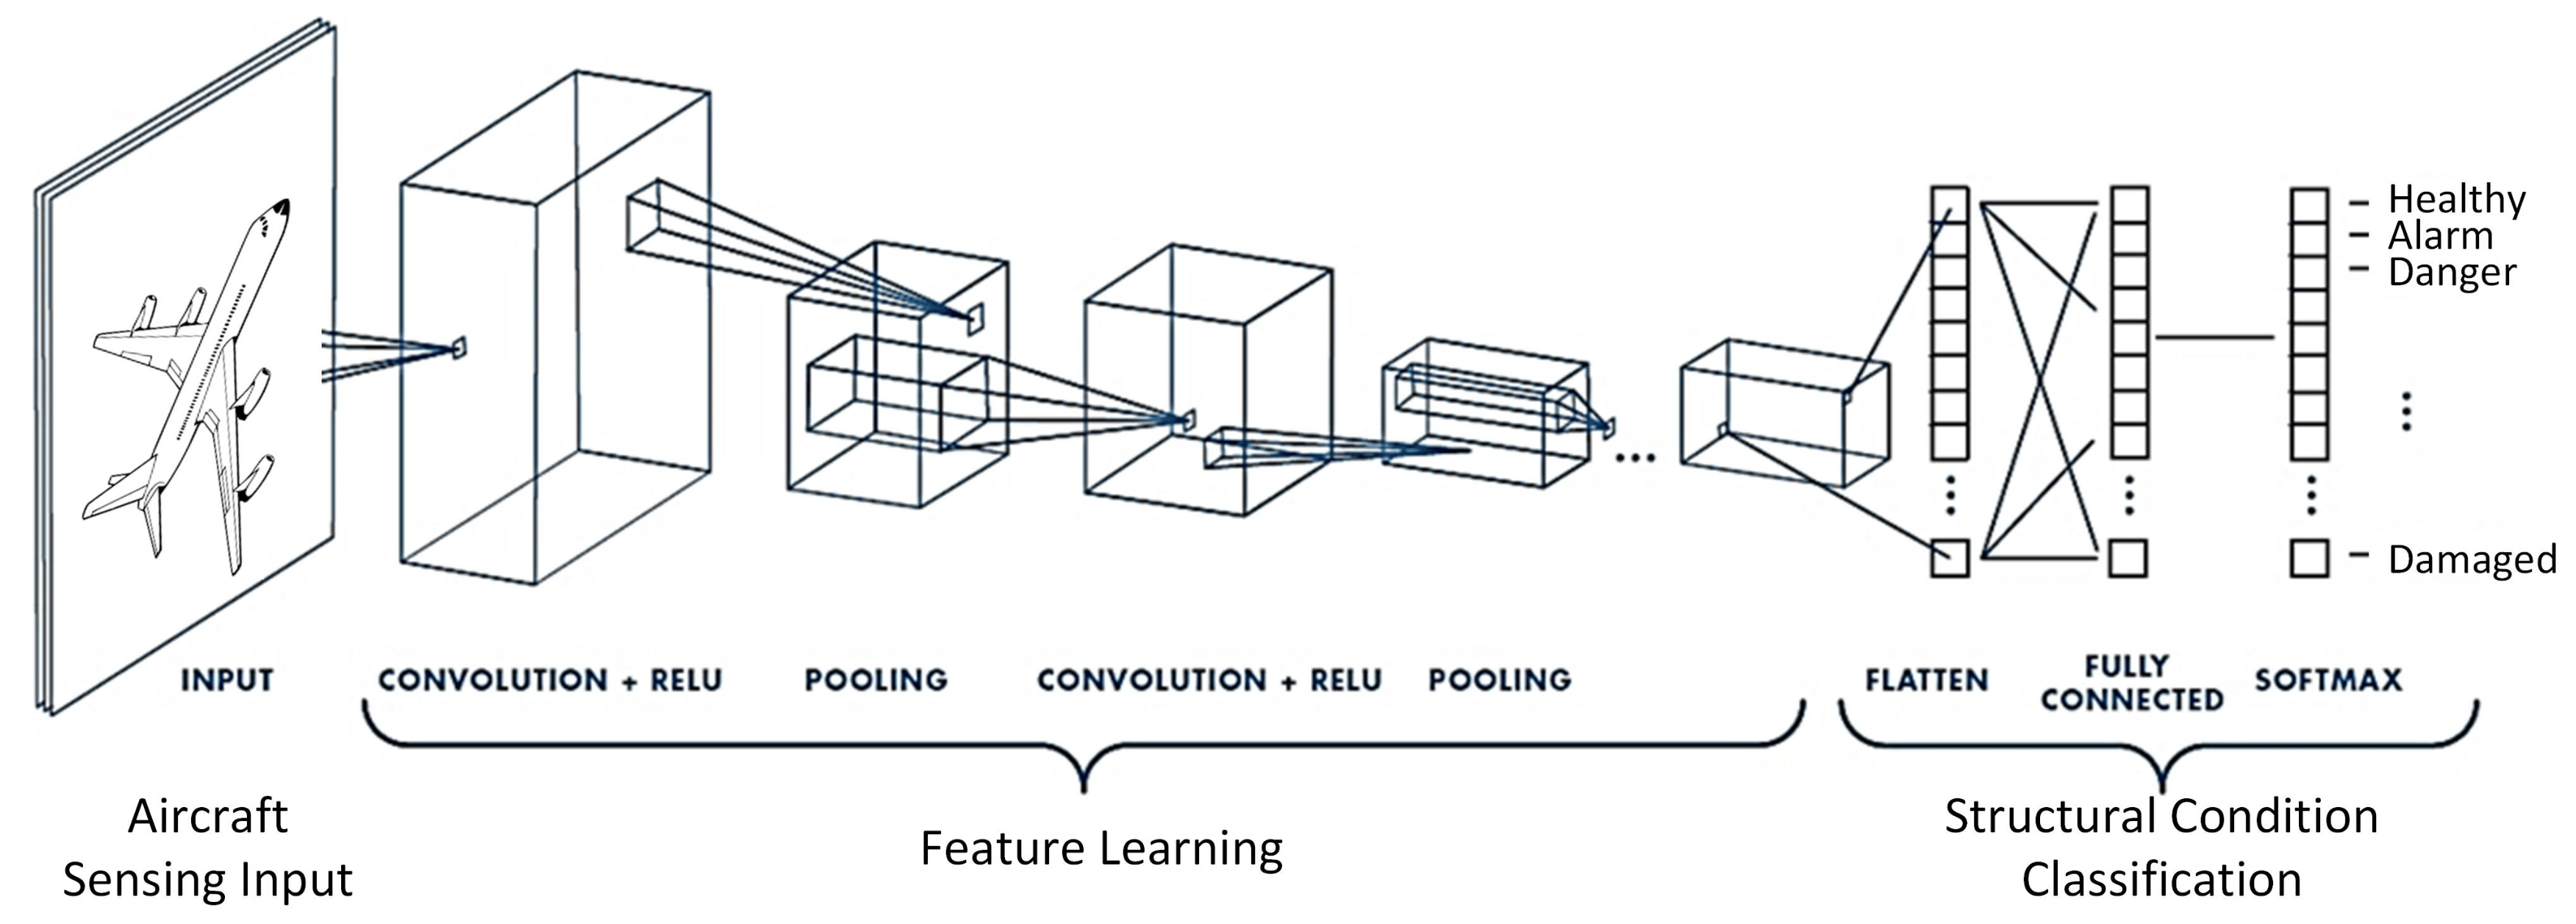
\includegraphics[scale=0.12]{gambar/arsitekturcnn.png}
    % Keterangan gambar yang diinputkan
    \caption{Arsitektur pada \emph{Convolutional Neural Network}}
    % Label referensi dari gambar yang diinputkan
    \label{fig:arsitektur cnn}
\end{figure}

Input CNN merupakan array tiga dimensi dengan ukuran seperti pada Persamaan 2.1. Apabila input merupakan suatu citra maka citra tersebut harus diubah menjadi array dua dimensi. 

% Persamaan 2.1
\begin{equation}
Baris * Kolom * Depth
\end{equation}

\emph{Convolution Layer} digunakan untuk menyaring (\emph{filter}) matriks dari citra \emph{input}. \emph{Zero Padd-ing} akan diperlukan untuk mempertahankan ukuran matriks dari citra \parencite{dwitama2019klasifikasi}. Ukuran kernel yang digunakan pada layer konvolusi adalah \(3 \times 3\) dan \(5 \times 5\). \emph{Output} dari lapisan konvolusi ini akan digunakan sebagai \emph{input} pada \emph{Pooling Layer} \parencite{hakim2018penerapan}. Apabila output dari \emph{Convolution Layer} bernilai negatif maka akan dilakukan perhitungan tambahan berupa aktifasi ReLU. Fungsi aktivasi ReLU akan nilai matriks yang bernilai negatif menjadi nol. Contoh penerapan dari aktivasi ReLU dapat dilihat pada Gambar 2.2.

% Gambar 2.2
\begin{figure} [ht] \centering
    % Nama dari file gambar yang diinputkan
    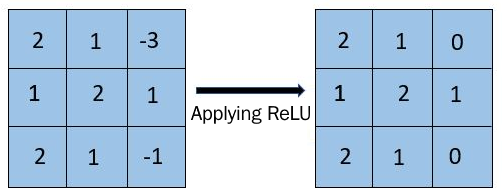
\includegraphics[scale=1]{gambar/aktivasiReLU.png}
    % Keterangan gambar yang diinputkan
    \caption{\emph{Aktivasi ReLU}}
    % Label referensi dari gambar yang diinputkan
    \label{fig:Aktivasi ReLU}
\end{figure}

\emph{Pooling Layer} digunakan untuk mengurangi jumlah parameter ketika ukuran citra terlalu besar dengan cara mengurangi dimensi setiap fitur. Karena ukuran citra menjadi lebih kecil maka proses \emph{feature map} akan menjadi lebih cepat \parencite{hakim2018penerapan}. \emph{Max Pooling} dilakukan dengan cara mengambil nilai dengan elemen terbesar sesuai dengan ukuran filter. Sebagai contoh pada Gambar 2.3 merupakan \emph{max pooling} dengan filter \(2 \times 2\) dengan \emph{stride} sebesar 2.

% Gambar 2.3
\begin{figure} [ht] \centering
    % Nama dari file gambar yang diinputkan
    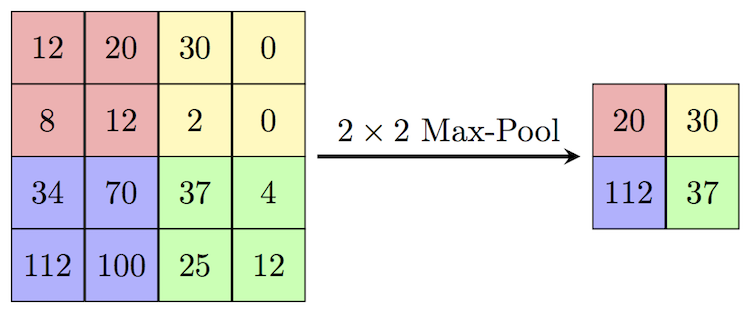
\includegraphics[scale=1.5]{gambar/maxPooling.png}
    % Keterangan gambar yang diinputkan
    \caption{\emph{Max Pooling}}
    % Label referensi dari gambar yang diinputkan
    \label{fig:Max Pooling}
\end{figure}

Flatten merupakan suatu proses dimana hasil dari \emph{Feature Learning} diubah menjadi vektor yang selanjutnya akan menjadi input pada proses klasifikasi dengan arsitektur \emph{fully connected layer}. Flatten digunakan untuk mengubah matriks menjadi vektor dengan menyesuaikan sesuai format \emph{input} pada \emph{neural network layer}. Flatten dapat digambarkan seperti pada Gambar 2.4.

% Gambar 2.4
\begin{figure} [ht] \centering
    % Nama dari file gambar yang diinputkan
    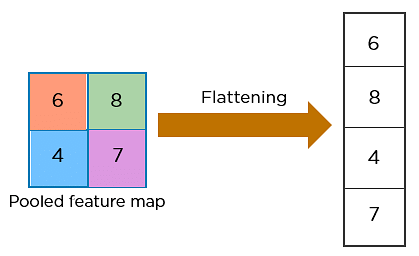
\includegraphics[scale=0.6]{gambar/flattening.png}
    % Keterangan gambar yang diinputkan
    \caption{Proses \emph{Flattening}}
    % Label referensi dari gambar yang diinputkan
    \label{fig:Proses Flattening}
\end{figure}

\newpage

\subsection{NVIDIA® Jetson Nano™}

% Gambar 2.1
\begin{figure} [ht] \centering
    % Nama dari file gambar yang diinputkan
    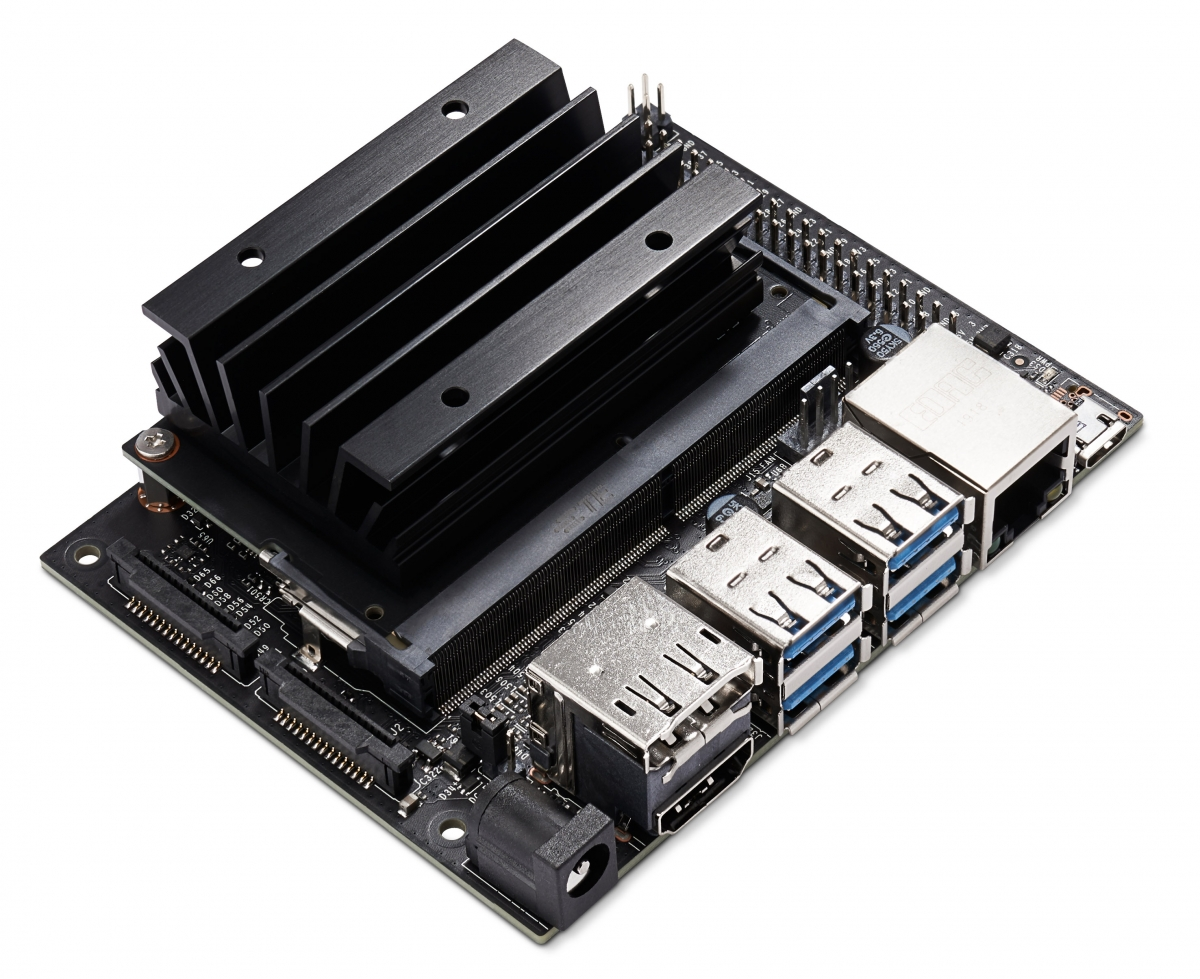
\includegraphics[scale=0.25]{gambar/JetsonNano.jpg}
    % Keterangan gambar yang diinputkan
    \caption{Perangkat Jetson Nano}
    % Label referensi dari gambar yang diinputkan
    \label{fig:Perangkat Jetson Nano}
\end{figure}

NVIDIA® Jetson Nano™ Developer Kit adalah komputer kecil dan kuat yang dapat digunakan untuk menjalankan beberapa \emph{neural network} secara paralel untuk berbagai penerapan seperti klasifikasi gambar, deteksi objek, segmentasi, dan pemrosesan ucapan. Semuanya dikemas dalam platform yang mudah digunakan dan hanya membutuhkan daya 5 watt \parencite{Developer_2023}.

Perangkat ini memiliki pin \emph{input} serta \emph{output} yang berlimpah, mulai dari GPIO hingga pin CSI. Jumlah pin yang berlimpah ini sangat memudahkan para pengembang dalam menghubung-kan berbagai perangkat tambahan seperti sensor untuk keperluan pengembangan aplikasi \emph{Artificial Intelligence}. NVIDIA® Jetson Nano™ Developer Kit juga didukung dengan NVIDIA JetPack yang mencakup berbagai perangkat lunak seperti Sistem Operasi Linux, cuDNN, NVIDIA CUDA, TensorRT, dan juga \emph{Board Support Package} (BSP) yang digunakan untuk keperluan \emph{Deep Learning} serta visi komputer.
\cleardoublepage

% Bab 3 desain dan implementasi
\chapter{METODOLOGI}
\label{chap:metodologi}

% Ubah bagian-bagian berikut dengan isi dari desain dan implementasi

Penelitian ini dilaksanakan sesuai dengan desain sistem berikut ini beserta implementasinya. Desain sistem merupakan konsep dari pembuatan dan perencangan infrastruktur dan kemudian diwujudkan dalam bentuk blok-blok alur yang harus dikerjakan.

\section{Deskripsi Sistem}
\label{sec:deskripsisistem}

Tugas akhir ini merupakan penelitian yang mengintegrasikan teknologi visi komputer agar dapat mengontrol gerak kursi roda. Secara umum penelitian kali ini akan menggunakan desain sistem sesuai dengan Gambar 3.1.

% Gambar 3.1
\begin{figure} [ht] \centering
    % Nama dari file gambar yang diinputkan
    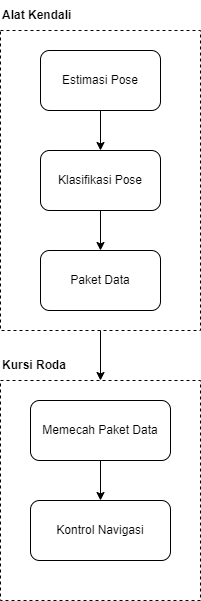
\includegraphics[scale=0.68]{gambar/blokDiagram.png}
    % Keterangan gambar yang diinputkan
    \caption{Blok Diagram Penelitian}
    % Label referensi dari gambar yang diinputkan
    \label{fig:Metodologi Penelitian}
\end{figure}

\subsection{Estimasi Pose}
Deteksi pose merupakan suatu proses yang melibatkan penggunaan bahasa pemrograman Python bersama dengan \emph{library} OpenCV dan \emph{framework} Mediapipe. Dalam konteks ini, Mediapipe berperan penting dalam mendapatkan informasi titik-titik \emph{landmark} yang signifikan pada objek yang diidentifikasi. \emph{Landmark} ini kemudian menjadi dasar untuk membentuk suatu representasi visual yang memvisualisasikan pose tersebut. Proses selanjutnya melibatkan penghubungan titik-titik \emph{landmark} yang telah ditentukan, di mana garis-garis dibuat untuk menggambarkan relasi spasial antar titik-titik tersebut. Dengan demikian, prosedur ini tidak hanya mengandalkan Mediapipe sebagai \emph{framework} utama, tetapi juga memanfaatkan OpenCV sebagai alat bantu untuk analisis citra dan manipulasi visual yang diperlukan dalam deteksi pose.

Pada penelitian kali ini akan memanfaatkan teknologi \emph{hand pose} dari Mediapipe untuk mengontrol gerak kursi roda. Terdapat beberapa titik \emph{keypoints} yang akan digunakan pada estimasi pose ini. Titik \emph{keypoints} yang akan digunakan pada estimasi  pose ini dapat dilihat pada Tabel 3.1.

\begin{table}[H]
\centering
    \caption{Tabel titik \emph{keypoints} yang relevan pada tahap estimasi pose}
    \label{tbl:titik keypoints}
    \begin{tabular}{|c|c|}
        \hline
        Nomor Keypoint & Nama Keypoint      \\ \hline
        0              & Pergelangan Tangan \\ \hline
        1              & CMC Ibu Jari       \\ \hline
        2              & MPM Ibu Jari       \\ \hline
        3              & IP Ibu Jari        \\ \hline
        4              & TIP Ibu Jari       \\ \hline
        5              & MCP Telunjuk       \\ \hline
        6              & PIP Telunjuk       \\ \hline
        7              & DIP Telunjuk       \\ \hline
        8              & TIP Telunjuk       \\ \hline
        9              & MCP Jari Tengah    \\ \hline
        10             & PIP Jari Tengah    \\ \hline
        11             & DIP Jari Tengah    \\ \hline
        12             & TIP Jari Tengah    \\ \hline
        13             & MCP Jari Manis     \\ \hline
        14             & PIP Jari Manis     \\ \hline
        15             & DIP Jari Manis     \\ \hline
        16             & TIP Jari Manis     \\ \hline
        17             & MCP Kelingking     \\ \hline
        18             & PIP Kelingking     \\ \hline
        19             & DIP Kelingking     \\ \hline
        20             & TIP Kelingking     \\ \hline
    \end{tabular}
\end{table}

Setiap titik \emph{landmark} yang terdapat pada peraga akan diwarnai dengan warna yang unik untuk membedakan setiap jarinya. Secara spesifik, warna yang diberikan pada setiap titik \emph{landmark} mencerminkan asosiasi dengan jari tertentu, sehingga menciptakan representasi visual yang lebih terperinci dan informatif. Untuk memberikan gambaran yang lebih konkret maka berikut ini contoh citra yang telah diestimasi pose yang dapat dilihat pada Gambar 3.2.

% Gambar 3.2
\begin{figure} [ht] \centering
    % Nama dari file gambar yang diinputkan
    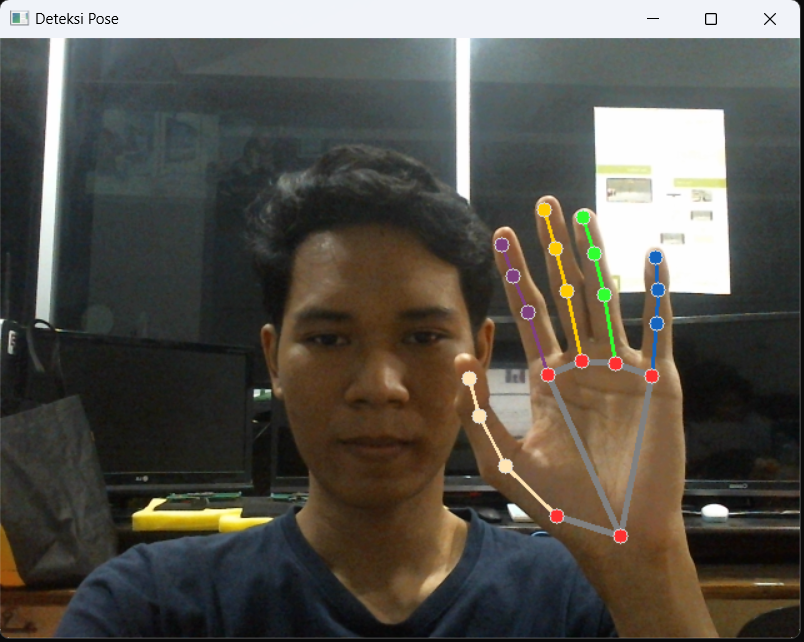
\includegraphics[scale=0.9]{gambar/bab3/EstimasiPose.png}
    % Keterangan gambar yang diinputkan
    \caption{Contoh citra yang telah diestimasi pose}
    % Label referensi dari gambar yang diinputkan
    \label{fig:contoh citra yang telah diestimasi pose}
\end{figure}

\subsection{Klasifikasi Pose}
Setelah proses estimasi pose tangan selsai, maka langkah selanjutnya ada mengelompokkan citra-citra hasil estimasi menjadi suatu dataset. Dataset ini akan memiliki 5 kelas berbeda yang masing-masing merepresentasikan perintah untuk maju, mundur, bergerak ke kanan, bergerak ke kiri, dan berhenti. Kelas ini mewakili perintah dasar untuk menggerakkan kursi roda. 

Untuk meningkatkan kinerja dan akurasi maka dataset ini kemudian akan melewati proses \emph{training} menggunakan algoritma \emph{Convolutional Neural Network} (CNN). Penggunaan CNN dalam \emph{training} dataset diharapkan dapat menghasilkan model yang mampu mengenali pola dan fitur yang kompleks, sehingga memungkinkan sistem untuk merespon dengan tepat terhadap variasi perintah yang mungkin diberikan oleh peraga. Hasil dari model prediksi yang telah dibuat dapat dilihat pada Tabel 3.2.

\newpage

% Tabel 3.2
\begin{table}[H]
\centering
    \caption{Tabel contoh klasifikasi citra}
    \label{tbl:contoh klasifikasi citra}
    \begin{tabular}{|c|c|}
        \hline
        Pose                & Citra              \\ \hline
        Kiri                & 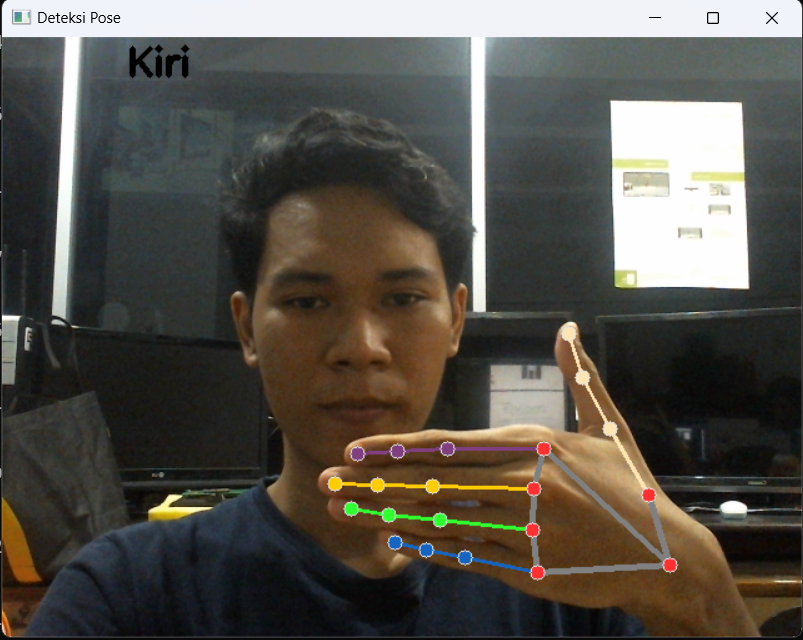
\includegraphics[scale=0.33]{gambar/bab3/Kiri.png}   \\ \hline
        Maju                & 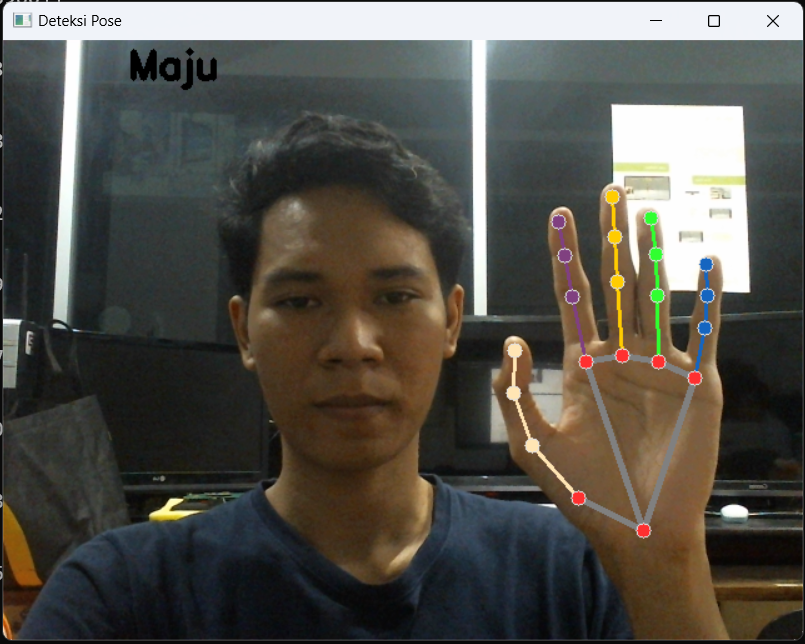
\includegraphics[scale=0.33]{gambar/bab3/Maju.png}   \\ \hline
        Stop                & 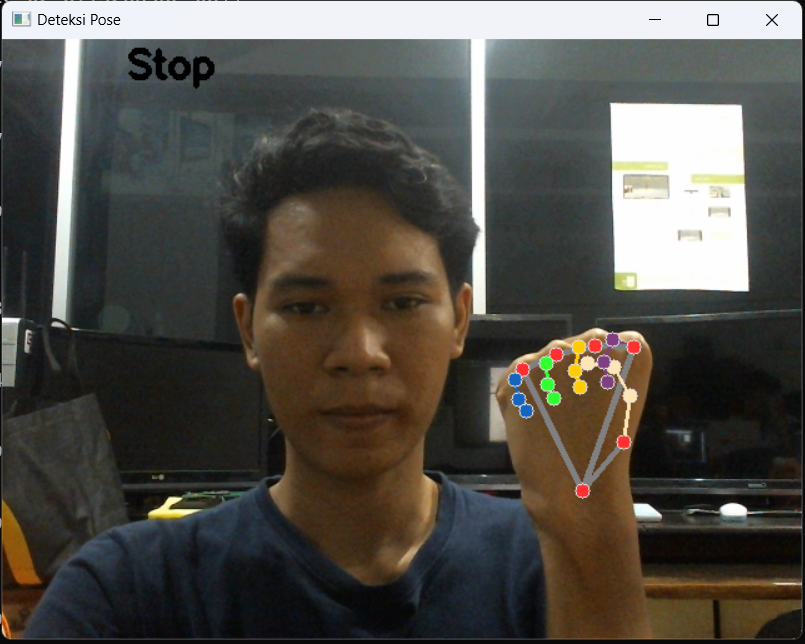
\includegraphics[scale=0.33]{gambar/bab3/Stop.png}   \\ \hline
        Mundur              & 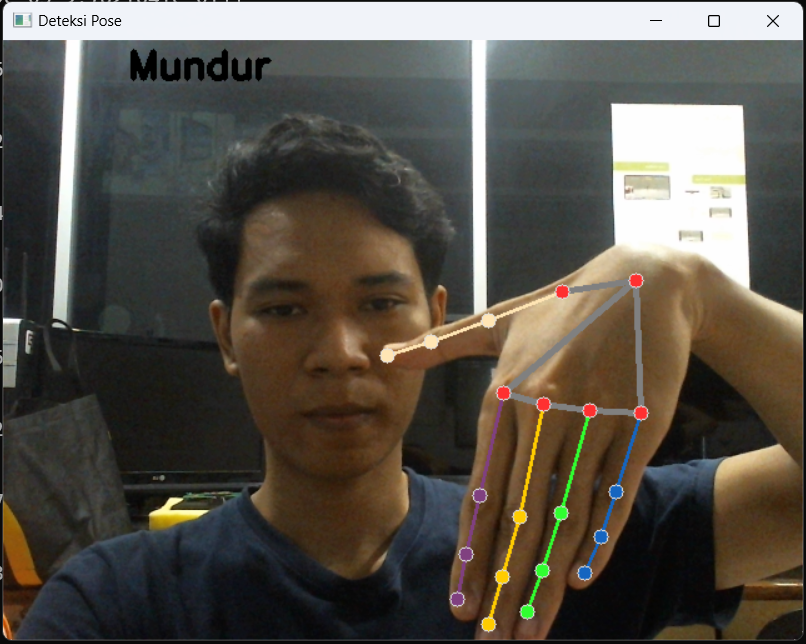
\includegraphics[scale=0.33]{gambar/bab3/Mundur.png} \\ \hline
        Kanan               & 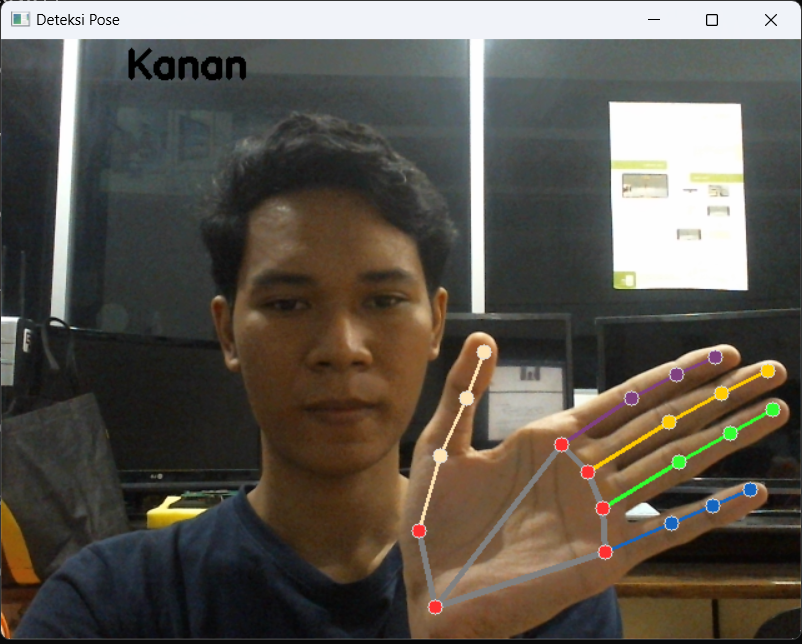
\includegraphics[scale=0.33]{gambar/bab3/Kanan.png}  \\ \hline
    \end{tabular}
\end{table}

\subsection{Paket Data}
Untuk dapat menggerakkan kursi roda maka perlu mengirimkan perintah ke kontroler kursi roda. Pada tahap klasifikasi pose telah didapatkan perintah dasar untuk menggerakkan kursi roda, seperti maju, mundur, kanan, kiri, maupun stop. Perintah ini kemudian akan digabungkan dengan kecepatan maksimal menjadi satu \emph{command} atau paket data seperti yang dilihat pada Persamaan 3.1.

% Persamaan 3.1
\begin{equation}
    Arah(char),Kecepatan(integer)
\end{equation}

Variabel arah memiliki tipe data \emph{char} yang akan menentukan gerak dari motor kursi roda, serta variabel kecepatan memiliki tipe data integer yang akan menentukan kecepatan maksimal dari kursi roda. Untuk memperkecil ukuran data maka kode instruksi untuk menentukan arah gerak menggunakan satu huruf untuk mewakili setiap gerakan. Kode instruksi dapat dilihat pada Tabel 3.2. 

% Tabel 3.2
\begin{table}[H]
\centering
    \caption{Kode instruksi dari hasil klasifikasi}
    \label{tbl:kode instruksi dari hasil klasifikasi}
    \begin{tabular}{|c|c|}
        \hline
        Klasifikasi Pose & Kode Instruksi \\ \hline
        Kiri             & A              \\ \hline
        Maju             & B              \\ \hline
        Stop             & C              \\ \hline
        Mundur           & D              \\ \hline
        Kanan            & E              \\ \hline
    \end{tabular}
\end{table}

Setelah kedua variabel tersebut digabungkan maka akan dikirim secara nirkabel, baik menggunakan Bluetooth maupun WiFi dari laptop atau Jetson Nano ke ESP32.

\subsection{Memecahkan Paket Data}
Paket data yang telah dikirimkan melalui laptop maupun Jetson Nano akan diterima oleh ESP32 menggunakan Bluetooth maupun WiFi. Saat diterima oleh ESP32, data tersebut akan menjalani serangkaian proses yang melibatkan pemecahan paket data dan penyesuaian sesuai dengan variabel yang telah ditentukan sebelumnya. Pemecahan paket data ini memungkinkan ESP32 untuk mendekomposisi informasi yang terkandung dalam setiap paket dan memastikan bahwa setiap variabel terpisah dengan akurat. Dengan demikian proses ini akan mengorganisir dan menyusun kembali informasi serta memastikan bahwa setiap variabel telah benar sesuai dengan nama variabel dan tipe data yang disediakan.

\subsection{Kontrol Navigasi}
Kedua variabel yang didapatkan dari pemecahan paket data akan diproses pada ESP32. Variabel arah akan berperan untuk menentukan arah gerak dari motor, sedangkan variabel kecepatan akan digunakan untuk menetapkan kecepatan maksimal dari pergerakan motor tersebut. Terdapat serangkaian logika \emph{if} berantai pada kontrol navigasi, dimana empat variabel dir akan menentukan arah putaran motor. Selain itu, nilai PWM maksimal dikonfigurasi dengan menggunakan variabel kecepatan sehingga pengguna dapat menyesuaikan kecepatan maksimal motor yang pengguna inginkan. Dengan demikian pada tahap ini ESP32 dapat secara efektif memproses data yang diterima melalui sistem nirkabel dan menghasilkan instruksi kontrol yang sesuai untuk menggerakkan kursi roda dengan arah dan kecepatan yang diinginkan.


\section{Implementasi Alat}
\label{sec:implementasi alat}

Pada penelitian ini dikembangkan suatu alat kontrol yang dapat menerima perintah melalui perangkat lain seperti laptop maupun Jetson Nano secara nirkabel. Pada sub bab ini akan dijabarkan implementasi dari alat yang dikembangkan pada penelitian ini.

\subsection{\emph{Hardware} dan \emph{Software} yang digunakan}
Berikut ini dijabarkan beberapa \emph{Hardware} dan juga \emph{Software} yang digunakan pada penelitian ini seperti berikut:
\begin{enumerate}
    \item Anaconda Navigator
    \item Arduino IDE 
    \item Laptop 
    \item Jetson Nano
    \item Kamera
    \item ESP32 Devkit V1
    \item 2 Kontroller Motor
    \item 2 DC-DC Voltage Regulator
    \item 2 DC Motor
    \item Baterai 24V
\end{enumerate}

\subsection{Skematik Alat}


Alat diimplementasikan dengan \lipsum[1]


\lipsum[2-3]

% Contoh input potongan kode dari file
\lstinputlisting[
  language=Python,
  caption={Program perhitungan bilangan prima.},
  label={lst:bilanganprima}
]{program/bilangan-prima.py}

\lipsum[4]

\cleardoublepage

% Bab 4 pengujian dan analisis
  \chapter{PENGUJIAN DAN ANALISIS}
\label{chap:pengujiananalisis}

% Ubah bagian-bagian berikut dengan isi dari pengujian dan analisis

Pada bab ini akan dipaparkan mengenai beberapa skenario pengujian sesuai dengan telah dijelaskan pada metodologi. Skenario pengujian ini dilakukan guna untuk mengetahui waktu \emph{delay} yang dibutuhkan untuk mentransmisikan data dari laptop menuju ESP32. Skenario yang nantinya akan diterapkan pada pengujian meliputi beberapa poin sebagai berikut:

\begin{enumerate}[nosep]
  \item Pengujian waktu \emph{delay} pengiriman data String melalui Bluetooth
  \item Pengujian waktu \emph{delay} pengiriman data JSON melalui Bluetooth
  \item Pengujian waktu \emph{delay} pengiriman data String melalui \emph{Access Point} WiFi
  \item Pengujian waktu \emph{delay} pengiriman data JSON melalui \emph{Access Point} WiFi
  \item Pengujian kestabilan Motor Kursi Roda
\end{enumerate}

Pelaksanaan metodologi serta skenario pengujian yang akan dipaparkan dalam bab ini diharapkan dapat memberikan pemahaman mengenai hasil dan pembahasan sehingga dapat ditarik kesimpulan dari Tugas Akhir yang telah dilaksanakan.


\section{Pengujian Waktu \emph{Delay} Pengiriman Data String Melalui Bluetooth}
\label{sec:delayBluetooth}

Pengujian waktu \emph{delay} pengiriman data ini dilakukan dengan cara mengirimkan data berupa string dari laptop menuju ESP32 melalui Bluetooth. Data yang dikirimkan adalah data arah dan kecepatan yang dipisahkan dengan koma seperti yang dapat dilihat pada Persamaan \ref{eq:string-2data}.

\begin{equation}
  \label{eq:string-2data}
    Arah,Kecepatan
\end{equation}

\begin{description}[nolistsep]
  \item[Keterangan]
  \item[Arah] : Variabel dengan tipe data \emph{char} yang digunakan untuk mengatur arah gerak motor kursi roda
  \item[Kecepatan] : Variabel dengan tipe data \emph{char} yang digunakan untuk mengatur kecepatan putar motor kursi roda 
\end{description}

Variabel arah memiliki tipe data \emph{char} yang digunakan untuk menentukan arah gerak dari motor kursi roda serta variabel kecepatan memiliki tipe data \emph{char} yang akan menentukan kecepatan maksimal dari rotasi motor kursi roda. Hasil dari pengujian waktu \emph{delay} pengiriman data string melalui bluetooth dapat dilihat pada Tabel \ref{tbl:delayBluetooth} dan Tabel \ref{tbl:delayBluetooth1}.

% Tabel 4.1
\begin{longtable}{|ccc|c|}
  \caption{Pengujian Waktu \emph{Delay} Pengiriman Data String Berisi 2 Nilai Melalui Bluetooth}
  \label{tbl:delayBluetooth}\\
  \hline
  \multicolumn{1}{|c|}{Data} & \multicolumn{1}{c|}{Timestamp Sent}  & Timestamp Received & Delay Time  \\ \hline
  \endfirsthead
  %
  \endhead
  %
  \multicolumn{1}{|c|}{A,S}  & \multicolumn{1}{c|}{22:35:51.523626} & 22:35:52.588       & 1,064374    \\ \hline
  \multicolumn{1}{|c|}{E,T}  & \multicolumn{1}{c|}{22:35:52.552591} & 22:35:53.591       & 1,038409    \\ \hline
  \multicolumn{1}{|c|}{E,P}  & \multicolumn{1}{c|}{22:35:53.565132} & 22:35:54.610       & 1,044868    \\ \hline
  \multicolumn{1}{|c|}{B,S}  & \multicolumn{1}{c|}{22:35:54.579935} & 22:35:55.602       & 1,022065    \\ \hline
  \multicolumn{1}{|c|}{D,U}  & \multicolumn{1}{c|}{22:35:55.593733} & 22:35:56.619       & 1,025267    \\ \hline
  \multicolumn{1}{|c|}{C,P}  & \multicolumn{1}{c|}{22:35:56.609782} & 22:35:57.624       & 1,014218    \\ \hline
  \multicolumn{1}{|c|}{A,R}  & \multicolumn{1}{c|}{22:35:57.618772} & 22:35:58.666       & 1,047228    \\ \hline
  \multicolumn{1}{|c|}{D,Q}  & \multicolumn{1}{c|}{22:39:03.614853} & 22:39:04.672       & 1,057147    \\ \hline
  \multicolumn{1}{|c|}{C,O}  & \multicolumn{1}{c|}{22:39:04.651688} & 22:39:05.690       & 1,038312    \\ \hline
  \multicolumn{1}{|c|}{B,T}  & \multicolumn{1}{c|}{22:39:05.666397} & 22:39:06.679       & 1,012603    \\ \hline
  \multicolumn{1}{|c|}{B,S}  & \multicolumn{1}{c|}{22:39:06.676370} & 22:39:07.711       & 1,03463     \\ \hline
  \multicolumn{1}{|c|}{B,T}  & \multicolumn{1}{c|}{22:39:07.686293} & 22:39:08.724       & 1,037707    \\ \hline
  \multicolumn{1}{|c|}{B,T}  & \multicolumn{1}{c|}{22:39:08.692595} & 22:39:09.729       & 1,036405    \\ \hline
  \multicolumn{1}{|c|}{C,O}  & \multicolumn{1}{c|}{22:41:01.427643} & 22:41:02.485       & 1,057357    \\ \hline
  \multicolumn{1}{|c|}{D,U}  & \multicolumn{1}{c|}{22:41:02.443022} & 22:41:03.486       & 1,042978    \\ \hline
  \multicolumn{1}{|c|}{A,U}  & \multicolumn{1}{c|}{22:41:03.449566} & 22:41:04.485       & 1,035434    \\ \hline
  \multicolumn{1}{|c|}{B,O}  & \multicolumn{1}{c|}{22:41:04.463072} & 22:41:05.507       & 1,043928    \\ \hline
  \multicolumn{1}{|c|}{D,O}  & \multicolumn{1}{c|}{22:41:05.470721} & 22:41:06.493       & 1,022279    \\ \hline
  \multicolumn{1}{|c|}{C,T}  & \multicolumn{1}{c|}{22:41:06.477458} & 22:41:07.512       & 1,034542    \\ \hline
  \multicolumn{1}{|c|}{B,U}  & \multicolumn{1}{c|}{22:41:07.492309} & 22:41:08.516       & 1,023691    \\ \hline
  \multicolumn{1}{|c|}{D,R}  & \multicolumn{1}{c|}{22:41:08.499671} & 22:41:09.532       & 1,032329    \\ \hline
  \multicolumn{1}{|c|}{E,Q}  & \multicolumn{1}{c|}{22:41:09.509928} & 22:41:10.547       & 1,037072    \\ \hline
  \multicolumn{1}{|c|}{E,V}  & \multicolumn{1}{c|}{22:41:10.523644} & 22:41:11.563       & 1,039356    \\ \hline
  \multicolumn{1}{|c|}{C,U}  & \multicolumn{1}{c|}{22:43:11.001438} & 22:43:12.026       & 1,024562    \\ \hline
  \multicolumn{1}{|c|}{C,P}  & \multicolumn{1}{c|}{22:43:12.028891} & 22:43:13.072       & 1,043109    \\ \hline
  \multicolumn{1}{|c|}{A,T}  & \multicolumn{1}{c|}{22:43:13.035252} & 22:43:14.066       & 1,030748    \\ \hline
  \multicolumn{1}{|c|}{D,Q}  & \multicolumn{1}{c|}{22:43:14.044212} & 22:43:15.086       & 1,041788    \\ \hline
  \multicolumn{1}{|c|}{D,O}  & \multicolumn{1}{c|}{22:43:15.050093} & 22:43:16.087       & 1,036907    \\ \hline
  \multicolumn{1}{|c|}{C,V}  & \multicolumn{1}{c|}{22:44:38.377450} & 22:44:39.438       & 1,06055     \\ \hline
  \multicolumn{1}{|c|}{B,P}  & \multicolumn{1}{c|}{22:44:39.427390} & 22:44:40.461       & 1,03361     \\ \hline
  \multicolumn{3}{|c|}{Average Delay Time}                                               & 1,037115767 \\ \hline
  \end{longtable}

Tabel \ref{tbl:delayBluetooth} menampilkan pengiriman data string yang terdiri dari 2 nilai dan dipisahkan dengan simbol koma (","). Dalam pengujian kali ini, data dikirimkan sebanyak 30 kali secara berturut-turut. Setelah ESP32 menerima dan mengolah data maka Flag akan dikirimkan ke Laptop. Hal ini dilakukan agar ESP32 dapat menerima data dengan baik dan berhasil memisahkan dan memasukkan kedua nilai tersebut sesuai dengan variabel yang telah ditentukan. Hasil dari pengujian ini menunjukkan bahwa waktu pengiriman rata-rata dari laptop menuju ESP32 melalui Bluetooth adalah sebesar 1,037115767 detik.

% Tabel 4.2
\begin{longtable}{|ccc|c|}
  \caption{Pengujian Waktu \emph{Delay} Pengiriman Data String Berisi 1 Nilai Melalui Bluetooth}
  \label{tbl:delayBluetooth1}\\
  \hline
  \multicolumn{1}{|c|}{Data} & \multicolumn{1}{c|}{Timestamp Sent}  & Timestamp Received & Delay Time  \\ \hline
  \endfirsthead
  %
  \endhead
  %
  \multicolumn{1}{|c|}{B}    & \multicolumn{1}{c|}{22:17:58.360200} & 22:17:59.417       & 1,0568      \\ \hline
  \multicolumn{1}{|c|}{B}    & \multicolumn{1}{c|}{22:17:59.396644} & 22:18:00.426       & 1,029356    \\ \hline
  \multicolumn{1}{|c|}{B}    & \multicolumn{1}{c|}{22:18:00.411642} & 22:18:01.449       & 1,037358    \\ \hline
  \multicolumn{1}{|c|}{C}    & \multicolumn{1}{c|}{22:18:01.419172} & 22:18:02.461       & 1,041828    \\ \hline
  \multicolumn{1}{|c|}{E}    & \multicolumn{1}{c|}{22:18:02.431706} & 22:18:03.436       & 1,004294    \\ \hline
  \multicolumn{1}{|c|}{B}    & \multicolumn{1}{c|}{22:18:03.441714} & 22:18:04.487       & 1,045286    \\ \hline
  \multicolumn{1}{|c|}{A}    & \multicolumn{1}{c|}{22:18:04.452937} & 22:18:05.481       & 1,028063    \\ \hline
  \multicolumn{1}{|c|}{B}    & \multicolumn{1}{c|}{22:18:05.468058} & 22:18:06.502       & 1,033942    \\ \hline
  \multicolumn{1}{|c|}{C}    & \multicolumn{1}{c|}{22:18:06.475522} & 22:18:07.504       & 1,028478    \\ \hline
  \multicolumn{1}{|c|}{A}    & \multicolumn{1}{c|}{22:18:07.483055} & 22:18:08.508       & 1,024945    \\ \hline
  \multicolumn{1}{|c|}{C}    & \multicolumn{1}{c|}{22:19:35.549304} & 22:19:36.610       & 1,060696    \\ \hline
  \multicolumn{1}{|c|}{A}    & \multicolumn{1}{c|}{22:19:36.580394} & 22:19:37.624       & 1,043606    \\ \hline
  \multicolumn{1}{|c|}{B}    & \multicolumn{1}{c|}{22:19:37.587334} & 22:19:38.612       & 1,024666    \\ \hline
  \multicolumn{1}{|c|}{B}    & \multicolumn{1}{c|}{22:19:38.593528} & 22:19:39.645       & 1,051472    \\ \hline
  \multicolumn{1}{|c|}{E}    & \multicolumn{1}{c|}{22:19:39.605674} & 22:19:40.634       & 1,028326    \\ \hline
  \multicolumn{1}{|c|}{E}    & \multicolumn{1}{c|}{22:19:40.621872} & 22:19:41.643       & 1,021128    \\ \hline
  \multicolumn{1}{|c|}{A}    & \multicolumn{1}{c|}{22:19:41.633767} & 22:19:42.668       & 1,034233    \\ \hline
  \multicolumn{1}{|c|}{D}    & \multicolumn{1}{c|}{22:19:42.641717} & 22:19:43.675       & 1,033283    \\ \hline
  \multicolumn{1}{|c|}{E}    & \multicolumn{1}{c|}{22:19:43.650596} & 22:19:44.682       & 1,031404    \\ \hline
  \multicolumn{1}{|c|}{D}    & \multicolumn{1}{c|}{22:19:44.659460} & 22:19:45.698       & 1,03854     \\ \hline
  \multicolumn{1}{|c|}{A}    & \multicolumn{1}{c|}{22:20:22.820901} & 22:20:23.885       & 1,064099    \\ \hline
  \multicolumn{1}{|c|}{E}    & \multicolumn{1}{c|}{22:20:23.850953} & 22:20:24.900       & 1,049047    \\ \hline
  \multicolumn{1}{|c|}{B}    & \multicolumn{1}{c|}{22:20:24.867989} & 22:20:25.873       & 1,005011    \\ \hline
  \multicolumn{1}{|c|}{E}    & \multicolumn{1}{c|}{22:20:25.879869} & 22:20:26.919       & 1,039131    \\ \hline
  \multicolumn{1}{|c|}{C}    & \multicolumn{1}{c|}{22:20:26.890743} & 22:20:27.925       & 1,034257    \\ \hline
  \multicolumn{1}{|c|}{D}    & \multicolumn{1}{c|}{22:20:27.899877} & 22:20:28.944       & 1,044123    \\ \hline
  \multicolumn{1}{|c|}{B}    & \multicolumn{1}{c|}{22:20:28.911163} & 22:20:29.917       & 1,005837    \\ \hline
  \multicolumn{1}{|c|}{A}    & \multicolumn{1}{c|}{22:20:29.918844} & 22:20:30.969       & 1,050156    \\ \hline
  \multicolumn{1}{|c|}{E}    & \multicolumn{1}{c|}{22:20:30.945381} & 22:20:31.991       & 1,045619    \\ \hline
  \multicolumn{1}{|c|}{E}    & \multicolumn{1}{c|}{22:20:31.972686} & 22:20:32.994       & 1,021314    \\ \hline
  \multicolumn{3}{|c|}{Average Delay Time}                                               & 1,035209933 \\ \hline
  \end{longtable}

Tabel \ref{tbl:delayBluetooth1} menampilkan pengiriman data string yang terdiri dari 1 nilai, yaitu arah. Dalam pengujian kali ini, data dikirimkan sebanyak 30 kali secara berturut-turut tanpa penambahan waktu \emph{delay} setiap kali mengirimkan data. Setelah ESP32 menerima dan mengolah data maka Flag akan dikirimkan ke Laptop. Hal ini dilakukan agar ESP32 dapat menerima data dengan baik dan berhasil memisahkan dan memasukkan kedua nilai tersebut sesuai dengan variabel yang telah ditentukan. Hasil dari pengujian ini menunjukkan bahwa waktu pengiriman rata-rata dari laptop menuju ESP32 melalui Bluetooth adalah sebesar 1,035209933 detik.

Ditemukan perbedaan waktu \emph{delay} yang tidak terlalu signifikan antara proses pengiriman string yang mengandung 2 nilai dibandingkan dengan string yang hanya berisi 1 nilai. Saat mengirimkan string yang memuat 2 data, pengujian menunjukkan adanya waktu \emph{delay} sekitar 1,037115767 detik. Dalam perbandingan dengan pengujian yang melibatkan string 1 nilai, waktu \emph{delay} yang tercatat hanya sekitar 1,035209933 detik. Setelah ESP32 menerima dan mengolah data maka Flag akan dikirimkan ke Laptop. Hal ini dilakukan agar ESP32 dapat menerima data secara optimal. Oleh karena itu, dapat disimpulkan bahwa dalam konteks pengiriman data melalui Bluetooth, pengguna dapat mengirim data string baik yang berisi 1 nilai maupun data string yang berisi 2 nilai, karena perbedaan waktu delay yang tidak terlalu berbeda.

\newpage

\section{Pengujian Waktu \emph{Delay} Pengiriman Data JSON Melalui Bluetooth}
\label{sec:delayBluetoothJSON}

Pengujian waktu \emph{delay} pengiriman data ini dilakukan dengan cara mengirimkan data berupa JSON dari laptop menuju ESP32 melalui Bluetooth. Data yang dikirimkan adalah data arah dan kecepatan yang dirangkum menjadi JSON seperti yang dapat dilihat pada Persamaan \ref{eq:json-2data} dan juga JSON yang hanya berisikan data arah seperti pada Persamaan \ref{eq:json-1data}

\begin{equation}
  \label{eq:json-2data}
    \{'arah': kode-arah, 'kecepatan': level-kecepatan\}
\end{equation}

\begin{description}[nolistsep]
  \item[Keterangan]
  \item[arah] : Key yang digunakan untuk menyimpan nilai kode-arah
  \item[kecepatan] : Key yang digunakan untuk menyimpan nilai level-kecepatan
  \item[kode-arah] : Value dengan tipe data \emph{char} yang digunakan untuk mengatur arah gerak motor kursi roda
  \item[level-kecepatan] : Value dengan tipe data \emph{char} yang digunakan untuk mengatur kecepatan putar motor kursi roda 
\end{description}


\begin{equation}
  \label{eq:json-1data}
    \{'arah': kode-arah\}
\end{equation}

\begin{description}[nolistsep]
  \item[Keterangan]
  \item[arah] : Key yang digunakan untuk menyimpan nilai kode-arah
  \item[kode-arah] : Value dengan tipe data \emph{char} yang digunakan untuk mengatur arah gerak motor kursi roda
\end{description}

Data JSON terdiri dari 2 bagian, yaitu \emph{key} dan \emph{value}. Terdapat 2 \emph{key}, yaitu arah dan kecepatan. \emph{Key} arah berisi \emph{value} dengan tipe data char yang digunakan untuk menentukan arah gerak dari motor kursi roda dan \emph{key} kecepatan berisi \emph{value} dengan tipe data \emph{char} yang digunakan untuk menentukan kecepatan maksimal dari rotasi motor kursi roda. Hasil dari pengujian waktu \emph{delay} pengiriman data JSON dapat dilihat pada Tabel \ref{tbl:delayBluetoothJSON2} dan Tabel \ref{tbl:delayBluetoothJSON1}.

% Tabel 4.3
\begin{longtable}{|ccc|c|}
  \caption{Pengujian Waktu \emph{Delay} Pengiriman Data JSON Berisi 2 Nilai Melalui Bluetooth}
  \label{tbl:delayBluetoothJSON2}\\
  \hline
  \multicolumn{1}{|c|}{Data}                              & \multicolumn{1}{c|}{Timestamp Sent}  & Timestamp Received & Delay Time  \\ \hline
  \endfirsthead
  %
  \endhead
  %
  \multicolumn{1}{|c|}{\{'arah': 'A', 'kecepatan': 'W'\}} & \multicolumn{1}{c|}{00:15:50.714083} & 00:15:51.776       & 1,061917    \\ \hline
  \multicolumn{1}{|c|}{\{"arah": "D", "kecepatan": "T"\}} & \multicolumn{1}{c|}{00:15:51.747698} & 00:15:52.796       & 1,048302    \\ \hline
  \multicolumn{1}{|c|}{\{"arah": "E", "kecepatan": "S"\}} & \multicolumn{1}{c|}{00:15:52.756331} & 00:15:53.766       & 1,009669    \\ \hline
  \multicolumn{1}{|c|}{\{"arah": "D", "kecepatan": "V"\}} & \multicolumn{1}{c|}{00:15:53.768717} & 00:15:54.807       & 1,038283    \\ \hline
  \multicolumn{1}{|c|}{\{"arah": "B", "kecepatan": "W"\}} & \multicolumn{1}{c|}{00:15:54.784688} & 00:15:55.824       & 1,039312    \\ \hline
  \multicolumn{1}{|c|}{\{"arah": "D", "kecepatan": "Q"\}} & \multicolumn{1}{c|}{00:15:55.792741} & 00:15:56.841       & 1,048259    \\ \hline
  \multicolumn{1}{|c|}{\{"arah": "A", "kecepatan": "O"\}} & \multicolumn{1}{c|}{00:15:56.803679} & 00:15:57.848       & 1,044321    \\ \hline
  \multicolumn{1}{|c|}{\{"arah": "E", "kecepatan": "Q"\}} & \multicolumn{1}{c|}{00:15:57.809707} & 00:15:58.854       & 1,044293    \\ \hline
  \multicolumn{1}{|c|}{\{"arah": "A", "kecepatan": "T"\}} & \multicolumn{1}{c|}{00:15:58.828668} & 00:15:59.840       & 1,011332    \\ \hline
  \multicolumn{1}{|c|}{\{"arah": "B", "kecepatan": "U"\}} & \multicolumn{1}{c|}{00:15:59.837626} & 00:16:00.875       & 1,037374    \\ \hline
  \multicolumn{1}{|c|}{\{"arah": "A", "kecepatan": "V"\}} & \multicolumn{1}{c|}{00:16:00.852674} & 00:16:01.888       & 1,035326    \\ \hline
  \multicolumn{1}{|c|}{\{"arah": "C", "kecepatan": "Q"\}} & \multicolumn{1}{c|}{00:16:01.867249} & 00:16:02.895       & 1,027751    \\ \hline
  \multicolumn{1}{|c|}{\{"arah": "A", "kecepatan": "O"\}} & \multicolumn{1}{c|}{00:16:02.885202} & 00:16:03.932       & 1,046798    \\ \hline
  \multicolumn{1}{|c|}{\{"arah": "A", "kecepatan": "V"\}} & \multicolumn{1}{c|}{00:16:03.910200} & 00:16:04.953       & 1,0428      \\ \hline
  \multicolumn{1}{|c|}{\{"arah": "B", "kecepatan": "T"\}} & \multicolumn{1}{c|}{00:16:04.917273} & 00:16:05.962       & 1,044727    \\ \hline
  \multicolumn{1}{|c|}{\{"arah": "D", "kecepatan": "W"\}} & \multicolumn{1}{c|}{00:16:05.925647} & 00:16:06.947       & 1,021353    \\ \hline
  \multicolumn{1}{|c|}{\{"arah": "E", "kecepatan": "P"\}} & \multicolumn{1}{c|}{00:16:06.942693} & 00:16:07.981       & 1,038307    \\ \hline
  \multicolumn{1}{|c|}{\{"arah": "E", "kecepatan": "R"\}} & \multicolumn{1}{c|}{00:16:07.955136} & 00:16:09.004       & 1,048864    \\ \hline
  \multicolumn{1}{|c|}{\{"arah": "A", "kecepatan": "T"\}} & \multicolumn{1}{c|}{00:16:08.966673} & 00:16:10.013       & 1,046327    \\ \hline
  \multicolumn{1}{|c|}{\{"arah": "E", "kecepatan": "P"\}} & \multicolumn{1}{c|}{00:16:09.977653} & 00:16:11.029       & 1,051347    \\ \hline
  \multicolumn{1}{|c|}{\{"arah": "E", "kecepatan": "O"\}} & \multicolumn{1}{c|}{00:16:10.985241} & 00:16:12.033       & 1,047759    \\ \hline
  \multicolumn{1}{|c|}{\{"arah": "C", "kecepatan": "R"\}} & \multicolumn{1}{c|}{00:16:11.997910} & 00:16:13.010       & 1,01209     \\ \hline
  \multicolumn{1}{|c|}{\{'arah': 'A', 'kecepatan': 'V'\}} & \multicolumn{1}{c|}{02:33:35.225933} & 02:33:36.305       & 1,079067    \\ \hline
  \multicolumn{1}{|c|}{\{"arah": "D", "kecepatan": "U"\}} & \multicolumn{1}{c|}{02:33:36.263807} & 02:33:37.288       & 1,024193    \\ \hline
  \multicolumn{1}{|c|}{\{"arah": "A", "kecepatan": "R"\}} & \multicolumn{1}{c|}{02:33:37.274213} & 02:33:38.297       & 1,022787    \\ \hline
  \multicolumn{1}{|c|}{\{"arah": "C", "kecepatan": "W"\}} & \multicolumn{1}{c|}{02:33:38.309262} & 02:33:39.356       & 1,046738    \\ \hline
  \multicolumn{1}{|c|}{\{"arah": "B", "kecepatan": "U"\}} & \multicolumn{1}{c|}{02:33:39.324412} & 02:33:40.382       & 1,057588    \\ \hline
  \multicolumn{1}{|c|}{\{"arah": "A", "kecepatan": "O"\}} & \multicolumn{1}{c|}{02:33:40.394353} & 02:33:41.424       & 1,029647    \\ \hline
  \multicolumn{1}{|c|}{\{"arah": "B", "kecepatan": "T"\}} & \multicolumn{1}{c|}{02:33:41.411566} & 02:33:42.433       & 1,021434    \\ \hline
  \multicolumn{3}{|c|}{Average Delay Time}                                                                            & 1,038895345 \\ \hline
  \end{longtable}

Tabel \ref{tbl:delayBluetoothJSON2} menampilkan pengiriman JSON yang terdiri dari 2 \emph{key}-\emph{value}, yaitu arah dan kecepatan. Dalam pengujian kali ini, data dikirimkan sebanyak 29 kali secara berturut-turut. Setelah ESP32 menerima dan mengolah data maka Flag akan dikirimkan ke Laptop. Hal ini dilakukan agar ESP32 dapat menerima data dengan baik dan berhasil memisahkan (\emph{deserialize}) serta memasukkan kedua nilai tersebut sesuai dengan variabel yang telah ditentukan. Hasil dari pengujian ini menunjukkan bahwa waktu pengiriman rata-rata dari laptop menuju ESP32 melalui Bluetooth adalah sebesar 1,038895345 detik.

% Tabel 4.4
\begin{longtable}{|ccc|c|}
  \caption{Pengujian Waktu \emph{Delay} Pengiriman Data JSON Berisi 1 Nilai Melalui Bluetooth}
  \label{tbl:delayBluetoothJSON1}\\
  \hline
  \multicolumn{1}{|c|}{Data}            & \multicolumn{1}{c|}{Timestamp Sent}  & Timestamp Received & Delay Time  \\ \hline
  \endfirsthead
  %
  \endhead
  %
  \multicolumn{1}{|c|}{\{'arah': 'D'\}} & \multicolumn{1}{c|}{23:51:13.043594} & 23:51:14.086       & 1,042406    \\ \hline
  \multicolumn{1}{|c|}{\{"arah": "A"\}} & \multicolumn{1}{c|}{23:51:14.076700} & 23:51:15.105       & 1,0283      \\ \hline
  \multicolumn{1}{|c|}{\{"arah": "D"\}} & \multicolumn{1}{c|}{23:51:15.086795} & 23:51:16.117       & 1,030205    \\ \hline
  \multicolumn{1}{|c|}{\{"arah": "E"\}} & \multicolumn{1}{c|}{23:51:16.099483} & 23:51:17.140       & 1,040517    \\ \hline
  \multicolumn{1}{|c|}{\{"arah": "C"\}} & \multicolumn{1}{c|}{23:51:17.105868} & 23:51:18.149       & 1,043132    \\ \hline
  \multicolumn{1}{|c|}{\{"arah": "C"\}} & \multicolumn{1}{c|}{23:51:18.117818} & 23:51:19.166       & 1,048182    \\ \hline
  \multicolumn{1}{|c|}{\{"arah": "E"\}} & \multicolumn{1}{c|}{23:51:19.127469} & 23:51:20.146       & 1,018531    \\ \hline
  \multicolumn{1}{|c|}{\{"arah": "B"\}} & \multicolumn{1}{c|}{23:51:20.135577} & 23:51:21.166       & 1,030423    \\ \hline
  \multicolumn{1}{|c|}{\{"arah": "C"\}} & \multicolumn{1}{c|}{23:51:21.145479} & 23:51:22.190       & 1,044521    \\ \hline
  \multicolumn{1}{|c|}{\{"arah": "C"\}} & \multicolumn{1}{c|}{23:51:22.158915} & 23:51:23.176       & 1,017085    \\ \hline
  \multicolumn{1}{|c|}{\{"arah": "E"\}} & \multicolumn{1}{c|}{23:51:23.168461} & 23:51:24.180       & 1,011539    \\ \hline
  \multicolumn{1}{|c|}{\{"arah": "D"\}} & \multicolumn{1}{c|}{23:51:24.180958} & 23:51:25.207       & 1,026042    \\ \hline
  \multicolumn{1}{|c|}{\{"arah": "A"\}} & \multicolumn{1}{c|}{23:51:25.194500} & 23:51:26.199       & 1,0045      \\ \hline
  \multicolumn{1}{|c|}{\{"arah": "C"\}} & \multicolumn{1}{c|}{23:51:26.203449} & 23:51:27.244       & 1,040551    \\ \hline
  \multicolumn{1}{|c|}{\{"arah": "A"\}} & \multicolumn{1}{c|}{23:51:27.216460} & 23:51:28.254       & 1,03754     \\ \hline
  \multicolumn{1}{|c|}{\{"arah": "A"\}} & \multicolumn{1}{c|}{23:51:28.224202} & 23:51:29.260       & 1,035798    \\ \hline
  \multicolumn{1}{|c|}{\{"arah": "C"\}} & \multicolumn{1}{c|}{23:51:29.236461} & 23:51:30.280       & 1,043539    \\ \hline
  \multicolumn{1}{|c|}{\{"arah": "A"\}} & \multicolumn{1}{c|}{23:51:30.243411} & 23:51:31.287       & 1,043589    \\ \hline
  \multicolumn{1}{|c|}{\{"arah": "D"\}} & \multicolumn{1}{c|}{23:51:31.253768} & 23:51:32.293       & 1,039232    \\ \hline
  \multicolumn{1}{|c|}{\{"arah": "A"\}} & \multicolumn{1}{c|}{23:51:32.266472} & 23:51:33.301       & 1,034528    \\ \hline
  \multicolumn{1}{|c|}{\{"arah": "C"\}} & \multicolumn{1}{c|}{23:51:33.279736} & 23:51:34.327       & 1,047264    \\ \hline
  \multicolumn{1}{|c|}{\{"arah": "D"\}} & \multicolumn{1}{c|}{23:51:34.288698} & 23:51:35.332       & 1,043302    \\ \hline
  \multicolumn{1}{|c|}{\{"arah": "C"\}} & \multicolumn{1}{c|}{23:51:35.303347} & 23:51:36.345       & 1,041653    \\ \hline
  \multicolumn{1}{|c|}{\{"arah": "E"\}} & \multicolumn{1}{c|}{23:51:36.323448} & 23:51:37.351       & 1,027552    \\ \hline
  \multicolumn{1}{|c|}{\{"arah": "E"\}} & \multicolumn{1}{c|}{23:51:37.331450} & 23:51:38.357       & 1,02555     \\ \hline
  \multicolumn{1}{|c|}{\{"arah": "C"\}} & \multicolumn{1}{c|}{23:51:38.341408} & 23:51:39.383       & 1,041592    \\ \hline
  \multicolumn{1}{|c|}{\{"arah": "A"\}} & \multicolumn{1}{c|}{23:51:39.351443} & 23:51:40.356       & 1,004557    \\ \hline
  \multicolumn{1}{|c|}{\{"arah": "B"\}} & \multicolumn{1}{c|}{23:51:40.366713} & 23:51:41.412       & 1,045287    \\ \hline
  \multicolumn{1}{|c|}{\{"arah": "D"\}} & \multicolumn{1}{c|}{23:51:41.377986} & 23:51:42.415       & 1,037014    \\ \hline
  \multicolumn{1}{|c|}{\{"arah": "E"\}} & \multicolumn{1}{c|}{23:51:42.392035} & 23:51:43.421       & 1,028965    \\ \hline
  \multicolumn{1}{|c|}{\{"arah": "B"\}} & \multicolumn{1}{c|}{23:51:43.406513} & 23:51:44.431       & 1,024487    \\ \hline
  \multicolumn{1}{|c|}{\{"arah": "C"\}} & \multicolumn{1}{c|}{23:51:44.424451} & 23:51:45.464       & 1,039549    \\ \hline
  \multicolumn{1}{|c|}{\{"arah": "C"\}} & \multicolumn{1}{c|}{23:51:45.430967} & 23:51:46.477       & 1,046033    \\ \hline
  \multicolumn{1}{|c|}{\{"arah": "C"\}} & \multicolumn{1}{c|}{23:51:46.438140} & 23:51:47.486       & 1,04786     \\ \hline
  \multicolumn{1}{|c|}{\{"arah": "B"\}} & \multicolumn{1}{c|}{23:51:47.449801} & 23:51:48.476       & 1,026199    \\ \hline
  \multicolumn{1}{|c|}{\{"arah": "C"\}} & \multicolumn{1}{c|}{23:51:48.457089} & 23:51:49.496       & 1,038911    \\ \hline
  \multicolumn{1}{|c|}{\{"arah": "E"\}} & \multicolumn{1}{c|}{23:51:49.471782} & 23:51:50.496       & 1,024218    \\ \hline
  \multicolumn{1}{|c|}{\{"arah": "B"\}} & \multicolumn{1}{c|}{23:51:50.487487} & 23:51:51.525       & 1,037513    \\ \hline
  \multicolumn{1}{|c|}{\{"arah": "D"\}} & \multicolumn{1}{c|}{23:51:51.496917} & 23:51:52.538       & 1,041083    \\ \hline
  \multicolumn{1}{|c|}{\{"arah": "D"\}} & \multicolumn{1}{c|}{23:51:52.504746} & 23:51:53.528       & 1,023254    \\ \hline
  \multicolumn{1}{|c|}{\{"arah": "B"\}} & \multicolumn{1}{c|}{23:51:53.519392} & 23:51:54.569       & 1,049608    \\ \hline
  \multicolumn{1}{|c|}{\{"arah": "D"\}} & \multicolumn{1}{c|}{23:51:54.526676} & 23:51:55.555       & 1,028324    \\ \hline
  \multicolumn{1}{|c|}{\{"arah": "B"\}} & \multicolumn{1}{c|}{23:51:55.539415} & 23:51:56.571       & 1,031585    \\ \hline
  \multicolumn{1}{|c|}{\{"arah": "E"\}} & \multicolumn{1}{c|}{23:51:56.552679} & 23:51:57.576       & 1,023321    \\ \hline
  \multicolumn{3}{|c|}{Average Delay Time}                                                          & 1,033746386 \\ \hline
  \end{longtable}

Tabel \ref{tbl:delayBluetoothJSON1} menampilkan pengiriman JSON yang terdiri dari 1 \emph{key}-\emph{value}, yaitu arah. Dalam pengujian kali ini, data dikirimkan sebanyak 44 kali secara berturut-turut. Setelah ESP32 menerima dan mengolah data maka Flag akan dikirimkan ke Laptop. Hal ini dilakukan agar ESP32 dapat menerima data dengan baik dan berhasil memisahkan (\emph{deserialize}) serta memasukkan nilai tersebut sesuai dengan variabel yang telah ditentukan. Hasil dari pengujian ini menunjukkan waktu pengiriman rata-rata dari laptop menuju ESP32 melalui Bluetooth sebesar 1,033746386 detik.

Dari kedua cara pengujian tersebut, didapatkan bahwa waktu \emph{delay} antara proses pengiriman JSON yang mengandung 2 \emph{key}-\emph{value} dibandingkan dengan JSON yang hanya berisikan 1 \emph{key}-\emph{value} tidak terlalu signifikan. Saat mengirimkan JSON yang berisikan 2 \emph{key}-\emph{value}, pengujian menunjukkan adanya \emph{delay} sebesar 1,038895345 detik. Jika dibandingkan dengan pengujian yang mengirimkan JSON dengan 1 \emph{key}-\emph{value}, waktu \emph{delay} yang tercatat adalah sebesar 1,033746386 detik. Dapat disimpulkan bahwa dalam konteks pengiriman data melalui Bluetooth, maka pengguna dapat mengirimkan data JSON baik yang berisi 1 \emph{key}-\emph{value} maupun yang berisi 2 \emph{key}-\emph{value}, karena perbedaan \emph{delay} kedua teknik tersebut tidak terlalu berbeda.

\section{Pengujian Waktu \emph{Delay} Pengiriman Data String Melalui \emph{Access Point} WiFi}
\label{sec:delayWiFi}

Pengujian waktu \emph{delay} pengiriman data ini dilakukan dengan cara mengirimkan data berupa String dari laptop menuji ESP32 melalui WiFi. ESP32 diatur sebagai \emph{Access Point}. Data yang dikirimkan adalah data arah dan kecepatan yang dipisahkan dengan simbol koma seperti yang dapat dilihat pada Persamaan \ref{eq:string-2Data}

\begin{equation}
  \label{eq:string-2Data}
    Arah,Kecepatan
\end{equation}

\begin{description}[nolistsep]
  \item[Keterangan]
  \item[Arah] : Variabel dengan tipe data \emph{char} yang digunakan untuk mengatur arah gerak motor kursi roda
  \item[Kecepatan] : Variabel dengan tipe data \emph{char} yang digunakan untuk mengatur kecepatan putar motor kursi roda 
\end{description}

Variabel arah memiliki tipe data char yang digunakan untuk menentukan arah gerak dari motor kursi roda serta variabel kecepatan yang memiliki tipe data \emph{char} yang akan menentukan kecepatan maksimal dari rotasi motor kursi roda. Hasil dari pengujian waktu \emph{delay} pengiriman data String melalui WiFi dapat dilihat pada Tabel \ref{tbl:delayWiFi2} dan Tabel \ref{tbl:delayWiFi1}

% Tabel 4.5
\begin{longtable}{|ccc|c|}
  \caption{Pengujian Waktu \emph{Delay} Pengiriman Data String Berisi 2 Nilai Melalui \emph{Access Point} WiFi}
  \label{tbl:delayWiFi2}\\
  \hline
  \multicolumn{1}{|c|}{Data} & \multicolumn{1}{c|}{Timestamp Sent}  & Timestamp Received & Delay Time  \\ \hline
  \endfirsthead
  %
  \endhead
  %
  \multicolumn{1}{|c|}{A,Q}  & \multicolumn{1}{c|}{03:49:59.217022} & 03:50:00.256       & 1,038978    \\ \hline
  \multicolumn{1}{|c|}{D,S}  & \multicolumn{1}{c|}{03:50:00.232977} & 03:50:01.260       & 1,027023    \\ \hline
  \multicolumn{1}{|c|}{A,O}  & \multicolumn{1}{c|}{03:50:01.256289} & 03:50:02.301       & 1,044711    \\ \hline
  \multicolumn{1}{|c|}{B,Q}  & \multicolumn{1}{c|}{03:50:02.278635} & 03:50:03.317       & 1,038365    \\ \hline
  \multicolumn{1}{|c|}{A,P}  & \multicolumn{1}{c|}{03:50:03.303124} & 03:50:04.336       & 1,032876    \\ \hline
  \multicolumn{1}{|c|}{E,U}  & \multicolumn{1}{c|}{03:50:04.326652} & 03:50:05.374       & 1,047348    \\ \hline
  \multicolumn{1}{|c|}{B,U}  & \multicolumn{1}{c|}{03:50:05.365324} & 03:50:06.411       & 1,045676    \\ \hline
  \multicolumn{1}{|c|}{D,R}  & \multicolumn{1}{c|}{03:50:06.374651} & 03:50:07.413       & 1,038349    \\ \hline
  \multicolumn{1}{|c|}{B,U}  & \multicolumn{1}{c|}{03:50:07.403115} & 03:50:08.432       & 1,028885    \\ \hline
  \multicolumn{1}{|c|}{E,Q}  & \multicolumn{1}{c|}{03:50:08.422259} & 03:50:09.469       & 1,046741    \\ \hline
  \multicolumn{1}{|c|}{D,S}  & \multicolumn{1}{c|}{03:50:09.452763} & 03:50:10.486       & 1,033237    \\ \hline
  \multicolumn{1}{|c|}{A,Q}  & \multicolumn{1}{c|}{03:50:10.470206} & 03:50:11.489       & 1,018794    \\ \hline
  \multicolumn{1}{|c|}{B,V}  & \multicolumn{1}{c|}{03:50:11.513787} & 03:50:12.556       & 1,042213    \\ \hline
  \multicolumn{1}{|c|}{D,S}  & \multicolumn{1}{c|}{03:50:12.519142} & 03:50:13.559       & 1,039858    \\ \hline
  \multicolumn{1}{|c|}{B,U}  & \multicolumn{1}{c|}{03:50:13.547184} & 03:50:14.595       & 1,047816    \\ \hline
  \multicolumn{1}{|c|}{C,S}  & \multicolumn{1}{c|}{03:50:14.566997} & 03:50:15.588       & 1,021003    \\ \hline
  \multicolumn{1}{|c|}{D,R}  & \multicolumn{1}{c|}{03:50:15.600210} & 03:50:16.638       & 1,03779     \\ \hline
  \multicolumn{1}{|c|}{C,W}  & \multicolumn{1}{c|}{03:50:16.616353} & 03:50:17.645       & 1,028647    \\ \hline
  \multicolumn{1}{|c|}{E,O}  & \multicolumn{1}{c|}{03:50:17.628725} & 03:50:18.664       & 1,035275    \\ \hline
  \multicolumn{1}{|c|}{C,Q}  & \multicolumn{1}{c|}{03:50:18.640125} & 03:50:19.654       & 1,013875    \\ \hline
  \multicolumn{1}{|c|}{D,U}  & \multicolumn{1}{c|}{03:50:19.645720} & 03:50:20.695       & 1,04928     \\ \hline
  \multicolumn{1}{|c|}{E,T}  & \multicolumn{1}{c|}{03:50:20.652242} & 03:50:21.674       & 1,021758    \\ \hline
  \multicolumn{1}{|c|}{A,S}  & \multicolumn{1}{c|}{03:50:21.664690} & 03:50:22.708       & 1,04331     \\ \hline
  \multicolumn{1}{|c|}{B,T}  & \multicolumn{1}{c|}{03:50:22.668332} & 03:50:23.705       & 1,036668    \\ \hline
  \multicolumn{1}{|c|}{E,P}  & \multicolumn{1}{c|}{03:50:23.671113} & 03:50:24.716       & 1,044887    \\ \hline
  \multicolumn{1}{|c|}{E,S}  & \multicolumn{1}{c|}{03:50:24.677001} & 03:50:25.719       & 1,041999    \\ \hline
  \multicolumn{1}{|c|}{A,V}  & \multicolumn{1}{c|}{03:50:25.683752} & 03:50:26.717       & 1,033248    \\ \hline
  \multicolumn{1}{|c|}{E,U}  & \multicolumn{1}{c|}{03:50:26.692210} & 03:50:27.719       & 1,02679     \\ \hline
  \multicolumn{1}{|c|}{C,V}  & \multicolumn{1}{c|}{03:50:27.696829} & 03:50:28.738       & 1,041171    \\ \hline
  \multicolumn{1}{|c|}{C,U}  & \multicolumn{1}{c|}{03:50:28.715728} & 03:50:29.738       & 1,022272    \\ \hline
  \multicolumn{1}{|c|}{D,R}  & \multicolumn{1}{c|}{03:50:29.719687} & 03:50:30.740       & 1,020313    \\ \hline
  \multicolumn{1}{|c|}{B,U}  & \multicolumn{1}{c|}{03:50:30.725229} & 03:50:31.760       & 1,034771    \\ \hline
  \multicolumn{1}{|c|}{B,R}  & \multicolumn{1}{c|}{03:50:31.731151} & 03:50:32.778       & 1,046849    \\ \hline
  \multicolumn{3}{|c|}{Average Delay Time}                                               & 1,035478061 \\ \hline
  \end{longtable}

Tabel \ref{tbl:delayWiFi2} menampilkan pengiriman data string yang terdiri dari 2 nilai dan dipisahkan dengan simbol koma (","). Dalam pengujian kali ini, data dikirimkan sebanyak 33 kali secara berturut-turut. Setelah ESP32 menerima dan mengolah data maka Flag akan dikirimkan ke Laptop. Hal ini dilakukan agar ESP32 dapat menerima data dengan baik dan berhasil memisahkan dan memasukkan kedua nilai tersebut sesuai dengan variabel yang telah ditentukan. Hasil dari pengujian ini menunjukkan bahwa waktu pengiriman rata-rata dari laptop menuju ESP32 melalui WiFi adalah sebesar 1,035478061 detik.

% Tabel 4.6
\begin{longtable}{|ccc|c|}
  \caption{Pengujian Waktu \emph{Delay} Pengiriman Data String Berisi 1 Nilai Melalui \emph{Access Point} WiFi}
  \label{tbl:delayWiFi1}\\
  \hline
  \multicolumn{1}{|c|}{Data} & \multicolumn{1}{c|}{Timestamp Sent}  & Timestamp Received & Delay Time \\ \hline
  \endfirsthead
  %
  \endhead
  %
  \multicolumn{1}{|c|}{C}    & \multicolumn{1}{c|}{03:40:01.384466} & 03:40:02.417       & 1,032534   \\ \hline
  \multicolumn{1}{|c|}{B}    & \multicolumn{1}{c|}{03:40:02.390604} & 03:40:03.432       & 1,041396   \\ \hline
  \multicolumn{1}{|c|}{E}    & \multicolumn{1}{c|}{03:40:03.395418} & 03:40:04.429       & 1,033582   \\ \hline
  \multicolumn{1}{|c|}{A}    & \multicolumn{1}{c|}{03:40:04.399194} & 03:40:05.446       & 1,046806   \\ \hline
  \multicolumn{1}{|c|}{D}    & \multicolumn{1}{c|}{03:40:05.404434} & 03:40:06.444       & 1,039566   \\ \hline
  \multicolumn{1}{|c|}{D}    & \multicolumn{1}{c|}{03:40:06.408148} & 03:40:07.414       & 1,005852   \\ \hline
  \multicolumn{1}{|c|}{D}    & \multicolumn{1}{c|}{03:40:07.413181} & 03:40:08.460       & 1,046819   \\ \hline
  \multicolumn{1}{|c|}{E}    & \multicolumn{1}{c|}{03:40:08.417232} & 03:40:09.449       & 1,031768   \\ \hline
  \multicolumn{1}{|c|}{E}    & \multicolumn{1}{c|}{03:40:09.423408} & 03:40:10.467       & 1,043592   \\ \hline
  \multicolumn{1}{|c|}{E}    & \multicolumn{1}{c|}{03:40:10.428216} & 03:40:11.449       & 1,020784   \\ \hline
  \multicolumn{1}{|c|}{A}    & \multicolumn{1}{c|}{03:40:11.431451} & 03:40:12.495       & 1,063549   \\ \hline
  \multicolumn{1}{|c|}{E}    & \multicolumn{1}{c|}{03:40:12.453247} & 03:40:13.477       & 1,023753   \\ \hline
  \multicolumn{1}{|c|}{D}    & \multicolumn{1}{c|}{03:40:13.456520} & 03:40:14.496       & 1,03948    \\ \hline
  \multicolumn{1}{|c|}{E}    & \multicolumn{1}{c|}{03:40:14.463187} & 03:40:15.480       & 1,016813   \\ \hline
  \multicolumn{1}{|c|}{B}    & \multicolumn{1}{c|}{03:40:15.480592} & 03:40:16.512       & 1,031408   \\ \hline
  \multicolumn{1}{|c|}{E}    & \multicolumn{1}{c|}{03:40:16.485499} & 03:40:17.507       & 1,021501   \\ \hline
  \multicolumn{1}{|c|}{D}    & \multicolumn{1}{c|}{03:40:17.488464} & 03:40:18.512       & 1,023536   \\ \hline
  \multicolumn{1}{|c|}{C}    & \multicolumn{1}{c|}{03:40:18.493367} & 03:40:19.521       & 1,027633   \\ \hline
  \multicolumn{1}{|c|}{C}    & \multicolumn{1}{c|}{03:40:19.497250} & 03:40:20.543       & 1,04575    \\ \hline
  \multicolumn{1}{|c|}{A}    & \multicolumn{1}{c|}{03:40:20.502595} & 03:40:21.527       & 1,024405   \\ \hline
  \multicolumn{1}{|c|}{C}    & \multicolumn{1}{c|}{03:40:21.506182} & 03:40:22.547       & 1,040818   \\ \hline
  \multicolumn{1}{|c|}{D}    & \multicolumn{1}{c|}{03:40:22.511194} & 03:40:23.540       & 1,028806   \\ \hline
  \multicolumn{1}{|c|}{C}    & \multicolumn{1}{c|}{03:40:23.515176} & 03:40:24.547       & 1,031824   \\ \hline
  \multicolumn{1}{|c|}{C}    & \multicolumn{1}{c|}{03:40:24.520190} & 03:40:25.554       & 1,03381    \\ \hline
  \multicolumn{1}{|c|}{E}    & \multicolumn{1}{c|}{03:40:25.525565} & 03:40:26.574       & 1,048435   \\ \hline
  \multicolumn{1}{|c|}{E}    & \multicolumn{1}{c|}{03:40:26.529479} & 03:40:27.580       & 1,050521   \\ \hline
  \multicolumn{1}{|c|}{D}    & \multicolumn{1}{c|}{03:40:27.558203} & 03:40:28.596       & 1,037797   \\ \hline
  \multicolumn{1}{|c|}{B}    & \multicolumn{1}{c|}{03:40:28.564173} & 03:40:29.588       & 1,023827   \\ \hline
  \multicolumn{1}{|c|}{B}    & \multicolumn{1}{c|}{03:40:29.568581} & 03:40:30.600       & 1,031419   \\ \hline
  \multicolumn{1}{|c|}{B}    & \multicolumn{1}{c|}{03:40:30.571593} & 03:40:31.619       & 1,047407   \\ \hline
  \multicolumn{1}{|c|}{A}    & \multicolumn{1}{c|}{03:40:31.576199} & 03:40:32.612       & 1,035801   \\ \hline
  \multicolumn{1}{|c|}{C}    & \multicolumn{1}{c|}{03:40:32.579504} & 03:40:33.619       & 1,039496   \\ \hline
  \multicolumn{3}{|c|}{Average Delay Time}                                               & 1,03470275 \\ \hline
  \end{longtable}

Tabel \ref{tbl:delayWiFi1} menampilkan pengiriman data string yang terdiri dari 1 nilai, yaitu arah. Dalam pengujian kali ini, data dikirimkan sebanyak 32 kali secara berturut-turut. Setelah ESP32 menerima dan mengolah data maka Flag akan dikirimkan ke Laptop. Hasil dari pengujian ini menunjukkan bahwa waktu pengiriman rata-rata dari laptop menuju ESP32 melalui WiFi adalah sebesar 1,03470275 detik.

Ditemukan perbedaan waktu \emph{delay} yang cukup signifikan antara proses pengiriman string yang mengandung 2 nilai dibandingkan dengan string yang hanya berisikan 1 nilai. Saat mengirimkan string yang memuat 2 data, pengujian menunjukkan adanya waktu \emph{delay} sekitar 1.059681387 detik. Dalam perbandingan dengan pengujian yang melibatkan string dengan 1 nilai, waktu yang \emph{delay} yang tercatat hanya 0.03499708571 detik. Penting untuk diperhatikan bahwa terdapat kekurangan saat mengirimkan data string yang mengandung 2 nilai, yaitu adanya penambahan \emph{delay} sebesar 1.3 detik setiap kali pengiriman data dilakukan. Hal ini dilakukan agar ESP32 dapat menerima data secara optimal. Oleh karena itu, dapat disimpulkan bahwa dalam konteks pengiriman data melalui WiFi, lebih disarankan untuk mengirimkan string dengan hanya 1 nilai guna menghindari \emph{delay} tambahan yang dapat mempengaruhi efisiensi dan kecepatan transmiri data secara keseluruhan.

\section{Pengujian Waktu \emph{Delay} Pengiriman Data JSON Melalui \emph{Access Point} WiFi}
\label{sec:delayWiFiJSON}

Pengujian waktu \emph{delay} pengiriman data ini dilakukan dengan cara mengirimkan data berupa JSON dari laptop menuju ESP32 melalui WiFi. Data yang dikirimkan adalah data arah dan kecepatan yang dirangkum menjadi JSON seperti yang dapat dilihat pada Persamaan \ref{eq:json-2Data} dan Persamaan \ref{eq:json-1Data}. 

\begin{equation}
  \label{eq:json-2Data}
    \{'arah': kode-arah, 'kecepatan': level-kecepatan\}
\end{equation}

\begin{description}[nolistsep]
  \item[Keterangan]
  \item[arah] : Key yang digunakan untuk menyimpan nilai kode-arah
  \item[kecepatan] : Key yang digunakan untuk menyimpan nilai level-kecepatan
  \item[kode-arah] : Value dengan tipe data \emph{char} yang digunakan untuk mengatur arah gerak motor kursi roda
  \item[level-kecepatan] : Value dengan tipe data \emph{char} yang digunakan untuk mengatur kecepatan putar motor kursi roda 
\end{description}

\begin{equation}
  \label{eq:json-1Data}
    \{'arah': kode-arah\}
\end{equation}

\begin{description}[nolistsep]
  \item[Keterangan]
  \item[arah] : Key yang digunakan untuk menyimpan nilai kode-arah
  \item[kode-arah] : Value dengan tipe data \emph{char} yang digunakan untuk mengatur arah gerak motor kursi roda 
\end{description}

Data JSON terdiri dari 2 bagian, yaitu \emph{key} dan \emph{value}. Terdapat 2 \emph{key}, yaitu arah dan kecepatan. \emph{Key} arah berisi \emph{value} dengan tipe data char yang digunakan untuk menentukan arah gerak dari motor kursi roda dan \emph{key} kecepatan berisi \emph{value} dengan tipe data \emph{char} yang digunakan untuk menentukan kecepatan maksimal dari rotasi motor kursi roda. Hasil dari pengujian waktu \emph{delay} pengiriman data JSON dapat dilihat pada Tabel \ref{tbl:delayWiFiJSON} dan Tabel \ref{tbl:delayWiFiJSON1}.

% Tabel 4.7
\begin{longtable}{|ccc|c|}
  \caption{Pengujian Waktu \emph{Delay} Pengiriman Data JSON Berisi 2 Nilai Melalui \emph{Access Point} WiFi}
  \label{tbl:delayWiFiJSON}\\
    \hline
    \multicolumn{1}{|c|}{Data}                              & \multicolumn{1}{c|}{Timestamp Sent}  & Timestamp Received & Delay Time  \\ \hline
    \endfirsthead
    %
    \endhead
    %
    \multicolumn{1}{|c|}{\{'arah': 'C', 'kecepatan': 89\}}  & \multicolumn{1}{c|}{18:58:14.500967} & 18:58:15.534       & 1.033033    \\ \hline
    \multicolumn{1}{|c|}{\{'arah': 'C', 'kecepatan': 103\}} & \multicolumn{1}{c|}{18:58:16.001310} & 18:58:17.091       & 1.08969     \\ \hline
    \multicolumn{1}{|c|}{\{'arah': 'C', 'kecepatan': 164\}} & \multicolumn{1}{c|}{18:58:17.502196} & 18:58:18.550       & 1.047804    \\ \hline
    \multicolumn{1}{|c|}{\{'arah': 'A', 'kecepatan': 101\}} & \multicolumn{1}{c|}{18:58:19.002654} & 18:58:20.026       & 1.023346    \\ \hline
    \multicolumn{1}{|c|}{\{'arah': 'A', 'kecepatan': 152\}} & \multicolumn{1}{c|}{18:58:20.502992} & 18:58:21.537       & 1.034008    \\ \hline
    \multicolumn{1}{|c|}{\{'arah': 'A', 'kecepatan': 19\}}  & \multicolumn{1}{c|}{18:58:22.003740} & 18:58:23.042       & 1.03826     \\ \hline
    \multicolumn{1}{|c|}{\{'arah': 'A', 'kecepatan': 198\}} & \multicolumn{1}{c|}{18:58:23.504455} & 18:58:24.539       & 1.034545    \\ \hline
    \multicolumn{1}{|c|}{\{'arah': 'A', 'kecepatan': 211\}} & \multicolumn{1}{c|}{18:58:25.005622} & 18:58:26.045       & 1.039378    \\ \hline
    \multicolumn{1}{|c|}{\{'arah': 'E', 'kecepatan': 238\}} & \multicolumn{1}{c|}{18:58:26.506072} & 18:58:27.543       & 1.036928    \\ \hline
    \multicolumn{1}{|c|}{\{'arah': 'D', 'kecepatan': 30\}}  & \multicolumn{1}{c|}{18:58:28.006535} & 18:58:29.175       & 1.168465    \\ \hline
    \multicolumn{1}{|c|}{\{'arah': 'D', 'kecepatan': 112\}} & \multicolumn{1}{c|}{18:58:29.507104} & 18:58:30.532       & 1.024896    \\ \hline
    \multicolumn{1}{|c|}{\{'arah': 'D', 'kecepatan': 7\}}   & \multicolumn{1}{c|}{18:58:31.007617} & 18:58:32.011       & 1.003383    \\ \hline
    \multicolumn{1}{|c|}{\{'arah': 'C', 'kecepatan': 66\}}  & \multicolumn{1}{c|}{18:58:32.508185} & 18:58:33.547       & 1.038815    \\ \hline
    \multicolumn{1}{|c|}{\{'arah': 'A', 'kecepatan': 105\}} & \multicolumn{1}{c|}{18:58:34.008584} & 18:58:35.051       & 1.042416    \\ \hline
    \multicolumn{1}{|c|}{\{'arah': 'B', 'kecepatan': 117\}} & \multicolumn{1}{c|}{18:58:35.509099} & 18:58:36.526       & 1.016901    \\ \hline
    \multicolumn{1}{|c|}{\{'arah': 'D', 'kecepatan': 223\}} & \multicolumn{1}{c|}{18:58:37.009885} & 18:58:38.037       & 1.027115    \\ \hline
    \multicolumn{1}{|c|}{\{'arah': 'A', 'kecepatan': 245\}} & \multicolumn{1}{c|}{18:58:38.510667} & 18:58:39.515       & 1.004333    \\ \hline
    \multicolumn{1}{|c|}{\{'arah': 'A', 'kecepatan': 15\}}  & \multicolumn{1}{c|}{18:58:40.011508} & 18:58:41.050       & 1.038492    \\ \hline
    \multicolumn{1}{|c|}{\{'arah': 'D', 'kecepatan': 156\}} & \multicolumn{1}{c|}{18:58:41.512148} & 18:58:42.543       & 1.030852    \\ \hline
    \multicolumn{1}{|c|}{\{'arah': 'C', 'kecepatan': 118\}} & \multicolumn{1}{c|}{18:58:43.013213} & 18:58:44.048       & 1.034787    \\ \hline
    \multicolumn{1}{|c|}{\{'arah': 'B', 'kecepatan': 200\}} & \multicolumn{1}{c|}{18:58:44.514015} & 18:58:45.551       & 1.036985    \\ \hline
    \multicolumn{1}{|c|}{\{'arah': 'E', 'kecepatan': 159\}} & \multicolumn{1}{c|}{18:58:46.014630} & 18:58:47.027       & 1.01237     \\ \hline
    \multicolumn{1}{|c|}{\{'arah': 'D', 'kecepatan': 39\}}  & \multicolumn{1}{c|}{18:58:47.515394} & 18:58:48.522       & 1.006606    \\ \hline
    \multicolumn{1}{|c|}{\{'arah': 'C', 'kecepatan': 200\}} & \multicolumn{1}{c|}{18:58:49.015871} & 18:58:50.056       & 1.040129    \\ \hline
    \multicolumn{1}{|c|}{\{'arah': 'B', 'kecepatan': 179\}} & \multicolumn{1}{c|}{18:58:50.516719} & 18:58:51.543       & 1.026281    \\ \hline
    \multicolumn{1}{|c|}{\{'arah': 'E', 'kecepatan': 55\}}  & \multicolumn{1}{c|}{18:58:52.017064} & 18:58:53.062       & 1.044936    \\ \hline
    \multicolumn{1}{|c|}{\{'arah': 'E', 'kecepatan': 228\}} & \multicolumn{1}{c|}{18:58:53.518106} & 18:58:54.544       & 1.025894    \\ \hline
    \multicolumn{1}{|c|}{\{'arah': 'C', 'kecepatan': 38\}}  & \multicolumn{1}{c|}{18:58:55.018428} & 18:58:56.059       & 1.040572    \\ \hline
    \multicolumn{1}{|c|}{\{'arah': 'D', 'kecepatan': 38\}}  & \multicolumn{1}{c|}{18:58:56.518869} & 18:58:57.560       & 1.041131    \\ \hline
    \multicolumn{1}{|c|}{\{'arah': 'C', 'kecepatan': 192\}} & \multicolumn{1}{c|}{18:58:58.019668} & 18:58:59.065       & 1.045332    \\ \hline
    \multicolumn{1}{|c|}{\{'arah': 'E', 'kecepatan': 56\}}  & \multicolumn{1}{c|}{18:58:59.520195} & 18:59:00.557       & 1.036805    \\ \hline
    \multicolumn{3}{|c|}{Average Delay Time}                                                                            & 1.037564129 \\ \hline
\end{longtable}

Tabel \ref{tbl:delayWiFiJSON} menampilkan pengiriman JSON yang terdiri dari 2 \emph{key}-\emph{value}, yaitu arah dan kecepatan. Dalam pengujian kali ini, data dikirimkan sebanyak 31 kali secara berturut-turut dengan penambahan waktu \emph{delay} sebesar 1.5 detik setiap kali mengirimkan data. Hal ini dilakukan agar ESP32 dapat menerima data dengan baik dan berhasil memisahkan (\emph{deserialize}) serta memasukkan kedua nilai tersebut sesuai dengan variabel yang telah ditentukan. Hasil dari pengujian ini menunjukkan bahwa waktu pengiriman rata-rata dari laptop menuju ESP32 melalui Bluetooth adalah sebesar 1,037564129 detik.


% Tabel 4.8
\begin{longtable}{|ccc|c|}
  \caption{Pengujian Waktu \emph{Delay} Pengiriman Data JSON Berisi 1 Nilai Melalui \emph{Access Point} WiFi}
  \label{tbl:delayWiFiJSON1}\\
    \hline
    \multicolumn{1}{|c|}{Data}            & \multicolumn{1}{c|}{Timestamp Sent}  & Timestamp Received & Delay Time  \\ \hline
    \endfirsthead
    %
    \endhead
    %
    \multicolumn{1}{|c|}{\{'arah': 'C'\}} & \multicolumn{1}{c|}{22:27:11.678759} & 22:27:12.710       & 1.031241    \\ \hline
    \multicolumn{1}{|c|}{\{'arah': 'B'\}} & \multicolumn{1}{c|}{22:27:13.184177} & 22:27:14.233       & 1.048823    \\ \hline
    \multicolumn{1}{|c|}{\{'arah': 'C'\}} & \multicolumn{1}{c|}{22:27:14.698806} & 22:27:15.748       & 1.049194    \\ \hline
    \multicolumn{1}{|c|}{\{'arah': 'A'\}} & \multicolumn{1}{c|}{22:27:16.203611} & 22:27:17.215       & 1.011389    \\ \hline
    \multicolumn{1}{|c|}{\{'arah': 'C'\}} & \multicolumn{1}{c|}{22:27:17.715604} & 22:27:18.746       & 1.030396    \\ \hline
    \multicolumn{1}{|c|}{\{'arah': 'A'\}} & \multicolumn{1}{c|}{22:27:19.222435} & 22:27:20.228       & 1.005565    \\ \hline
    \multicolumn{1}{|c|}{\{'arah': 'C'\}} & \multicolumn{1}{c|}{22:27:20.730434} & 22:27:21.771       & 1.040566    \\ \hline
    \multicolumn{1}{|c|}{\{'arah': 'D'\}} & \multicolumn{1}{c|}{22:27:22.239679} & 22:27:23.285       & 1.045321    \\ \hline
    \multicolumn{1}{|c|}{\{'arah': 'C'\}} & \multicolumn{1}{c|}{22:27:23.750695} & 22:27:24.788       & 1.037305    \\ \hline
    \multicolumn{1}{|c|}{\{'arah': 'E'\}} & \multicolumn{1}{c|}{22:27:25.265167} & 22:27:26.301       & 1.035833    \\ \hline
    \multicolumn{1}{|c|}{\{'arah': 'C'\}} & \multicolumn{1}{c|}{22:27:26.769275} & 22:27:27.804       & 1.034725    \\ \hline
    \multicolumn{1}{|c|}{\{'arah': 'C'\}} & \multicolumn{1}{c|}{22:27:28.276680} & 22:27:29.317       & 1.04032     \\ \hline
    \multicolumn{1}{|c|}{\{'arah': 'D'\}} & \multicolumn{1}{c|}{22:27:29.789932} & 22:27:30.831       & 1.041068    \\ \hline
    \multicolumn{1}{|c|}{\{'arah': 'B'\}} & \multicolumn{1}{c|}{22:27:31.342439} & 22:27:32.400       & 1.057561    \\ \hline
    \multicolumn{1}{|c|}{\{'arah': 'B'\}} & \multicolumn{1}{c|}{22:27:32.848560} & 22:27:33.882       & 1.03344     \\ \hline
    \multicolumn{1}{|c|}{\{'arah': 'A'\}} & \multicolumn{1}{c|}{22:27:34.369849} & 22:27:35.396       & 1.026151    \\ \hline
    \multicolumn{1}{|c|}{\{'arah': 'C'\}} & \multicolumn{1}{c|}{22:27:35.877856} & 22:27:36.924       & 1.046144    \\ \hline
    \multicolumn{1}{|c|}{\{'arah': 'B'\}} & \multicolumn{1}{c|}{22:27:37.525218} & 22:27:38.531       & 1.005782    \\ \hline
    \multicolumn{1}{|c|}{\{'arah': 'A'\}} & \multicolumn{1}{c|}{22:27:39.043576} & 22:27:40.095       & 1.051424    \\ \hline
    \multicolumn{1}{|c|}{\{'arah': 'E'\}} & \multicolumn{1}{c|}{22:27:40.637793} & 22:27:41.671       & 1.033207    \\ \hline
    \multicolumn{1}{|c|}{\{'arah': 'B'\}} & \multicolumn{1}{c|}{22:27:42.143229} & 22:27:43.168       & 1.024771    \\ \hline
    \multicolumn{1}{|c|}{\{'arah': 'E'\}} & \multicolumn{1}{c|}{22:27:43.677645} & 22:27:44.714       & 1.036355    \\ \hline
    \multicolumn{1}{|c|}{\{'arah': 'D'\}} & \multicolumn{1}{c|}{22:27:45.218328} & 22:27:46.257       & 1.038672    \\ \hline
    \multicolumn{1}{|c|}{\{'arah': 'C'\}} & \multicolumn{1}{c|}{22:27:46.723402} & 22:27:47.758       & 1.034598    \\ \hline
    \multicolumn{1}{|c|}{\{'arah': 'B'\}} & \multicolumn{1}{c|}{22:27:48.296809} & 22:27:49.347       & 1.050191    \\ \hline
    \multicolumn{1}{|c|}{\{'arah': 'D'\}} & \multicolumn{1}{c|}{22:27:49.898938} & 22:27:50.940       & 1.041062    \\ \hline
    \multicolumn{1}{|c|}{\{'arah': 'B'\}} & \multicolumn{1}{c|}{22:27:51.405449} & 22:27:52.453       & 1.047551    \\ \hline
    \multicolumn{1}{|c|}{\{'arah': 'D'\}} & \multicolumn{1}{c|}{22:27:52.914479} & 22:27:53.965       & 1.050521    \\ \hline
    \multicolumn{1}{|c|}{\{'arah': 'E'\}} & \multicolumn{1}{c|}{22:27:54.458062} & 22:27:55.497       & 1.038938    \\ \hline
    \multicolumn{1}{|c|}{\{'arah': 'E'\}} & \multicolumn{1}{c|}{22:27:55.966855} & 22:27:57.010       & 1.043145    \\ \hline
    \multicolumn{1}{|c|}{\{'arah': 'E'\}} & \multicolumn{1}{c|}{22:27:57.472623} & 22:27:58.518       & 1.045377    \\ \hline
    \multicolumn{1}{|c|}{\{'arah': 'D'\}} & \multicolumn{1}{c|}{22:28:01.988199} & 22:28:03.032       & 1.043801    \\ \hline
    \multicolumn{1}{|c|}{\{'arah': 'C'\}} & \multicolumn{1}{c|}{22:28:03.502648} & 22:28:04.548       & 1.045352    \\ \hline
    \multicolumn{1}{|c|}{\{'arah': 'B'\}} & \multicolumn{1}{c|}{22:28:05.007693} & 22:28:06.048       & 1.040307    \\ \hline
    \multicolumn{1}{|c|}{\{'arah': 'C'\}} & \multicolumn{1}{c|}{22:28:07.635244} & 22:28:08.708       & 1.072756    \\ \hline
    \multicolumn{3}{|c|}{Average Delay Time}                                                          & 1.038824343 \\ \hline
\end{longtable}

Tabel \ref{tbl:delayWiFiJSON1} menampilkan pengiriman JSON yang terdiri dari 1 \emph{key}-\emph{value}, yaitu arah. Dalam pengujian kali ini, data dikirimkan sebanyak 35 kali secara berturut-turut dengan penambahan waktu \emph{delay} sebesar 1.5 detik setiap kali mengirimkan data. Hal ini dilakukan agar ESP32 dapat menerima data dengan baik dan berhasil memisahkan (\emph{deserialize}) serta memasukkan nilai tersebut sesuai dengan variabel yang telah ditentukan. Hasil dari pengujian ini menunjukkan waktu pengiriman rata-rata dari laptop menuju ESP32 melalui Bluetooth sebesar 1.038824343 detik.

Dari kedua cara pengujian tersebut, didapatkan bahwa waktu \emph{delay} antara proses pengiriman JSON yang mengandung 2 \emph{key}-\emph{value} dibandingkan dengan JSON yang hanya berisikan 1 \emph{key}-\emph{value} tidak terlalu signifikan. Saat mengirimkan JSON yang berisikan 2 \emph{key}-\emph{value}, pengujian menunjukkan adanya \emph{delay} sebesar 1,037564129 detik. Jika dibandingkan dengan pengujian yang mengirimkan JSON dengan 1 \emph{key}-\emph{value}, waktu \emph{delay} yang tercatat adalah sebesar 1.038824343 detik. Terdapat anomali pada pengujian ini, karena waktu delay pada saat mengirimkan data JSON yang berisikan 2 \emph{key}-\emph{value} lebih kecil jika dibandingkan dengan saat mengirimkan data JSON yang berisikan 1 \emph{key}-\emph{value} walaupun perbedaan waktu \emph{delay}-nya tidak terlalu signifikan.

\subsection{Pengujian Kestabilan Motor Kursi Roda}

Pengujian kestabilan motor dilakukan untuk mendeteksi derajat penyimpangan dari setiap motor. Pada pengujian ini akan dilakukan dengan cara menggerakkan kursi roda kearah depan (maju) dan juga kearah belakang (mundur). Perbedaan antara posisi akhir roda dengan titik pusat akan diukur untuk menentukan sudut penyimpangan seperti pada Gambar \ref{fig:DokumentasiJarakPenyimpangan}. Sudut Penyimpangan dapat dihitung menggunakan Persamaan \ref{eq:sudut-error}. Hasil dari pengujian ini dapat dilihat pada Tabel \ref{tbl:kestabilanmaju} dan Tabel \ref{tbl:kestabilanmundur}.

\begin{equation}
  \label{eq:sudut-error}
  Sudut Penyimpangan = \arctan \left ( \frac{Jarak Penyimpangan}{Jarak Tempuh} \right )
\end{equation}

\begin{description}[nolistsep]
  \item[Keterangan]
  \item[Sudut Penyimpangan] : Besar sudut penyimpangan gerak motor kursi roda (\textdegree)
  \item[Jarak Penyimpangan] : Jarak penyimpangan posisi akhir roda yang diukur dari posisi garis lurus jarak tempuh (cm)
  \item[Jarak Tempuh] : Lintasan garis lurus yang harus ditempuh oleh kursi roda (m)
\end{description}

\begin{longtable}{|ccc|c|}
  \caption{Pengujian Kestabilan Motor Kursi Roda Dengan Gerak Maju}
  \label{tbl:kestabilanmaju}\\
  \hline
  \multicolumn{1}{|c|}{\begin{tabular}[c]{@{}c@{}}Jarak \\ Tempuh\end{tabular}} & \multicolumn{1}{c|}{\begin{tabular}[c]{@{}c@{}}Jarak \\ Penyimpangan\end{tabular}} & \begin{tabular}[c]{@{}c@{}}Sudut\\ Penyimpangan\end{tabular} & \begin{tabular}[c]{@{}c@{}}Arah\\ Penyimpangan\end{tabular} \\ \hline
  \endfirsthead
  %
  \endhead
  %
  \multicolumn{1}{|c|}{10,34}                                                   & \multicolumn{1}{c|}{47}                                                            & 2,60\textdegree                                              & Kiri                                                        \\ \hline
  \multicolumn{1}{|c|}{10,50}                                                   & \multicolumn{1}{c|}{49}                                                            & 2,67\textdegree                                              & Kiri                                                        \\ \hline
  \multicolumn{1}{|c|}{10,74}                                                   & \multicolumn{1}{c|}{53}                                                            & 2,83\textdegree                                              & Kiri                                                        \\ \hline
  \multicolumn{1}{|c|}{10,53}                                                   & \multicolumn{1}{c|}{51}                                                            & 2,77\textdegree                                              & Kiri                                                        \\ \hline
  \multicolumn{1}{|c|}{10,62}                                                   & \multicolumn{1}{c|}{57}                                                            & 3,07\textdegree                                              & Kiri                                                        \\ \hline
  \multicolumn{3}{|c|}{Sudut Penyimpangan Rata - Rata}                                                                                                                                                                              & 2,788\textdegree                                            \\ \hline
  \end{longtable}

Tabel \ref{tbl:kestabilanmaju} menampilkan hasil pengujian kestabilan motor kursi roda dengan gerak maju. Pengujian ini dilakukan sebanyak 5 kali dengan jarak tempuh bervariasi dan lebih dari 10 meter. Hasil dari pengujian ini menunjukkan bahwa kursi roda cenderung bergerak kearah kiri dengan rata-rata sudut penyimpangan sebesar 2,788\textdegree.

\begin{longtable}{|ccc|c|}
  \caption{Pengujian Kestabilan Motor Kursi Roda Dengan Gerak Mundur}
  \label{tbl:kestabilanmundur}\\
  \hline
  \multicolumn{1}{|c|}{\begin{tabular}[c]{@{}c@{}}Jarak \\ Tempuh\end{tabular}} & \multicolumn{1}{c|}{\begin{tabular}[c]{@{}c@{}}Jarak \\ Penyimpangan\end{tabular}} & \begin{tabular}[c]{@{}c@{}}Sudut\\ Penyimpangan\end{tabular} & \begin{tabular}[c]{@{}c@{}}Arah\\ Penyimpangan\end{tabular} \\ \hline
  \endfirsthead
  %
  \endhead
  %
  \multicolumn{1}{|c|}{10,17}                                                   & \multicolumn{1}{c|}{102}                                                           & 5,73\textdegree                                              & Kanan                                                       \\ \hline
  \multicolumn{1}{|c|}{10,33}                                                   & \multicolumn{1}{c|}{96}                                                            & 5.31\textdegree                                              & Kanan                                                       \\ \hline
  \multicolumn{1}{|c|}{10,24}                                                   & \multicolumn{1}{c|}{91}                                                            & 5,08\textdegree                                              & Kanan                                                       \\ \hline
  \multicolumn{1}{|c|}{10,67}                                                   & \multicolumn{1}{c|}{107}                                                           & 5,73\textdegree                                              & Kanan                                                       \\ \hline
  \multicolumn{1}{|c|}{10,46}                                                   & \multicolumn{1}{c|}{103}                                                           & 5,62\textdegree                                              & Kanan                                                       \\ \hline
  \multicolumn{3}{|c|}{Sudut Penyimpangan Rata - Rata}                                                                                                                                                                              & 5,494\textdegree                                            \\ \hline
  \end{longtable}

  Tabel \ref{tbl:kestabilanmundur} menampilkan hasil pengujian kestabilan motor kursi roda dengan gerak mundur. Pengujian ini dilakukan sebanyak 5 kali dengan jarak tempuh bervariasi dan lebih dari 10 meter. Hasil dari pengujian ini menunjukkan bahwa kursi roda cenderung bergerak kearah kanan dengan rata-rata sudut penyimpangan sebesar 5,494\textdegree.
\cleardoublepage

% Bab 5 penutup
\chapter{PENUTUP}
\label{chap:penutup}

Pada bab ini akan dipaparkan kesimpulan dari hasil pengujian yang akan menjawab dari permasalahan yang diangkat dari pelaksanaan tugas akhir ini. Pada bab ini juga diapaprkan saran mengenai hal yang dapat dilakukan untuk mengembangkan penelitian kedepannya.

% Ubah bagian-bagian berikut dengan isi dari penutup

\section{Kesimpulan}
\label{sec:kesimpulan}

Berdasarkan hasil pengujian yang dilakukan selama pelaksanaan tugas akhir ini adalah sebagai berikut:

\begin{enumerate}[nolistsep]

  \item Waktu \emph{delay} rata-rata terendah terdapat pada pengujian dengan mengirimkan string dengan 1 nilai dan ditransmisikan melalui WiFi. Waktu \emph{delay} rata-ratanya adalah sebesar 0,03499708571 detik.

  \item Waktu \emph{delay} rata-rata tertinggi terdapat pada pengujian dengan mengirimkan string dengan 2 nilai dan ditransmisikan melalui WiFi. Waktu \emph{delay} rata-ratanya adalah sebesar 1,059681387 detik.
  
  \item Waktu \emph{delay} tambahan pada program pengirim data diperlukan untuk beberapa pengujian. Hal ini diakibatkan agar tidak terjadi penumpukan (\emph{flooding}) data yang dapat mengganggu kinerja dari ESP32.

  \item Terdapat beberapa pengujian yang memerlukan waktu \emph{delay} tambahan pada program pengirim data seperti pada pengiriman data String berisi 2 nilai melalui Bluetooth yang memerlukan waktu \emph{delay} tambahan sebesar 1,5 detik, pengiriman data JSON dengan 2 nilai melalui Bluetooth yang memerlukan waktu \emph{delay} tambahan sebesar 1,1 detik, pengiriman data String berisi 2 nilai melalui WiFi yang memerlukan waktu \emph{delay} tambahan sebesar 1,3 detik, pengiriman data JSON yang berisi 2 nilai melalui WiFi yang memerlukan waktu \emph{delay} tambahan sebesar 1,5 detik, pengiriman data JSON yang berisi 1 nilai melalui Bluetooth yang memerlukan waktu \emph{delay} tambahan sebesar 1 detik, pengiriman data JSON yang berisi 1 nilai melalui WiFi yang memerlukan waktu \emph{delay} tambahan sebesar 1,5 detik.
  
  \item Hanya 2 pengujian yang tidak memerlukan waktu \emph{delay} tambahan pada program pengirim data, yaitu pada pengiriman data String yang berisi 1 nilai melalui Bluetooth dan pengiriman data String yang berisi 1 nilai melalui WiFi. 
  
  \item Data yang ditransmisikan untuk mengontrol kursi roda melalui visi komputer lebih baik menggunakan String yang hanya berisi 1 nilai, yaitu variabel arah yang dianalogikan dengan 1 karakter huruf. 
  
  \item Transmisi data yang digunakan untuk mengontrol kursi roda melalui visi komputer lebih baik menggunakan WiFi dengan ESP32 sebagai \emph{Access Point}-nya.

\end{enumerate}

\section{Saran}
\label{chap:saran}

Berdasarkan hasil yang diperoleh dari penelitian ini maka saran yang dapat dipertimbangkan untuk pengembangan lebih lanjut adalah sebagai berikut:

\begin{enumerate}[nolistsep]

  \item Kecepatan putar motor diatur melalui ESP32 dengan menggunakan \emph{button} ataupun potensiometer.

  \item Mencoba menggunakan gestur lain untuk mengontrol gerak kursi roda.

\end{enumerate}

\cleardoublepage

\chapter*{DAFTAR PUSTAKA}
\addcontentsline{toc}{chapter}{DAFTAR PUSTAKA}
\renewcommand\refname{}
\vspace{2ex}
\renewcommand{\bibname}{}
\begingroup
\def\chapter*#1{}
\printbibliography
\endgroup
\cleardoublepage

\chapter*{LAMPIRAN}
\cleardoublepage


% Biografi penulis
\begin{center}
  \Large
  \textbf{BIOGRAFI PENULIS}
\end{center}

\addcontentsline{toc}{chapter}{BIOGRAFI PENULIS}

\vspace{2ex}

\begin{wrapfigure}{L}{0.3\textwidth}
  \centering
  \vspace{-3ex}
  % Ubah file gambar berikut dengan file foto dari mahasiswa
  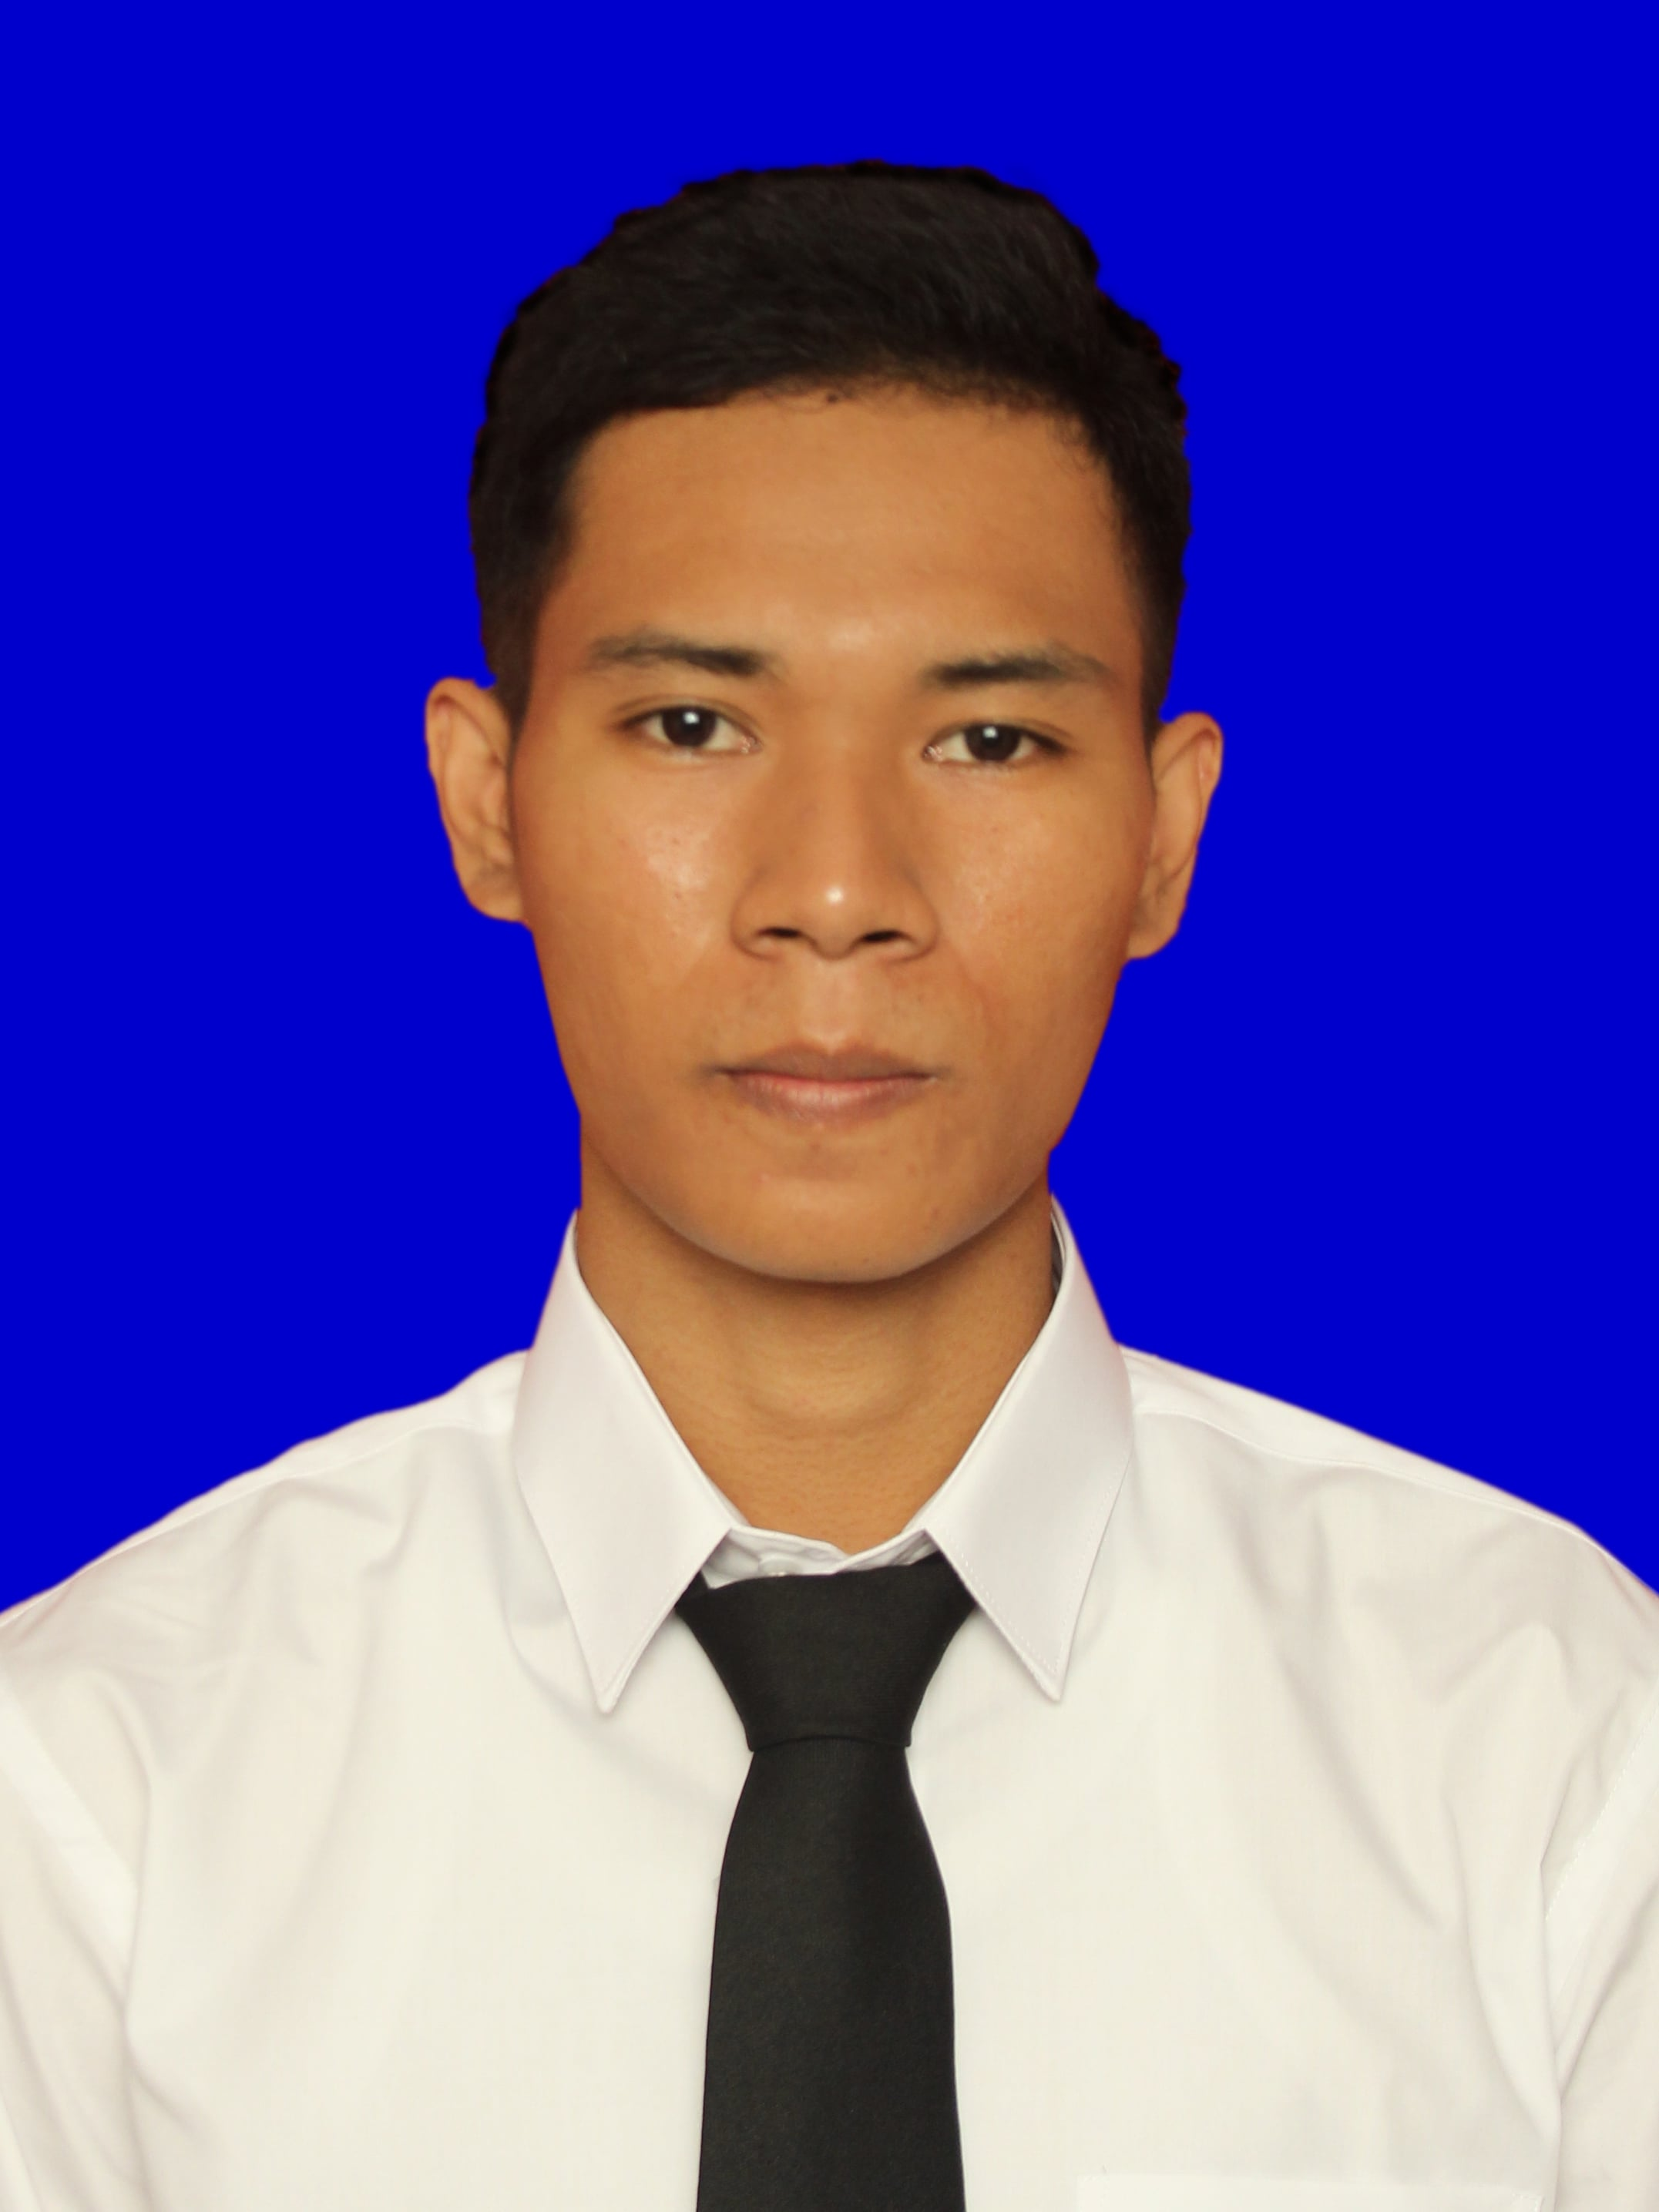
\includegraphics[width=0.3\textwidth]{gambar/HarisSetiadi.jpg}
  \vspace{-4ex}
\end{wrapfigure}

% Ubah kalimat berikut dengan biografi dari mahasiswa
\name{}, atau yang biasa dikenal dengan Haris, lahir pada tanggal 21 Maret 2000 di kota Denpasar. Penulis merupakan anak pertama dari tiga bersaudara yang tinggal dan besar di Denpasar, Bali. Setelah lulus dari SMA Negeri 2 Denpasar, penulis kemudian melanjutkan pendidikan ke jenjang strata satu di Departemen Teknik Komputer, Fakultas Teknologi Elektro dan Informatika Cerdas, Institut Teknologi Sepuluh Nopember mulai tahun 2019. 

Penulis merupakan orang yang aktif berorganisasi, dan memiliki berbagai \emph{softskill} serta \emph{hardskill}. Hal ini dibuktikan dengan rekam jejak organisasi dan kepanitiaan dari penulis seperti, Wakil Kepala Departemen Pengabdian Masyarakat Tim Pembina Kerohanian Hindu (TPKH-ITS), Wakil Ketua Internal pada TPKH Festival 2021, Staff Generasi Baru Indonesia (GenBI ITS), Staff Himpunan Mahasiswa Teknik Komputer (HIMATEKKOM ITS), hingga menjadi \emph{Product Manager} salah satu kelompok pada Bootcamp MyDigitalAcademy yang diselenggarakan oleh Bank Mandiri.
\cleardoublepage

\end{document}
